\chapter{Black hole formation 1: dust collapse}
\label{s:lem}

\minitoc

\section{Introduction}

After having investigated black holes in equilibrium, via the
Schwarzschild and Kerr solutions, we move to dynamical black holes,
more specifically to the standard process of
black hole formation: \emph{gravitational collapse}\index{gravitational!collapse}.
To deal with analytical solutions, we simplify the problem as much as
possible. First we assume spherical symmetry, which is quite natural
as a first approximation for modeling the gravitational collapse
of a stellar core or a gas cloud. A drawback is that this forbids the
study of gravitational waves\index{gravitational!waves}, since by
virtue of Birkhoff's theorem\index{Birkhoff's theorem} (to be proven in this chapter)
the exterior
of any spherically symmetric collapsing object is a piece of Schwarzschild
spacetime, i.e. it does not contain any gravitational radiation.
The second major approximation is to consider \emph{pressureless matter},
commonly referred to as \emph{dust}\index{dust}.

We start by deriving from Einstein's equation the system of partial differential
equations yielding the metric for spherically symmetric dust (Lemaître-Tolman
system) and write down the most general solutions (Sec.~\ref{s:lem:LT_equat}).
Then we specialize these solutions to the case of a homogeneous ball of dust
collapsing from rest (Oppenheimer-Snyder collapse, Sec.~\ref{s:lem:OS}),
which we study in details, in particular regarding the birth of the event
horizon and the existence of trapped surfaces. Finally, we consider
the observational appearance of the gravitational collapse and the black hole
formation to a remote observer (Sec.~\ref{s:lem:obs}).



\section{Lemaître-Tolman equations} \label{s:lem:LT_equat}

\subsection{Hypotheses} \label{s:lem:hyp}

As mentioned in the Introduction, we shall restrict ourselves to
spherically symmetric\footnote{See Sec.~\ref{s:sch:static_spher} for the precise
definition of \emph{spherically symmetric}.} spacetimes, and for concreteness, to 4-dimensional ones. The most general spherically symmetric 4-dimensional spacetime $(\M,\w{g})$
can be described in terms of coordinates $(x^\alpha)=(\tau,\chi,\th,\ph)$ such that
the metric tensor writes
\be \label{e:lem:metric_sync_coord}
    \w{g} = - \dd\tau^2 + a(\tau,\chi)^2 \dd\chi^2
        + r(\tau,\chi)^2 \left( \dd\th^2 + \sin^2\th\, \dd\ph^2 \right)  ,
\ee
where $a(\tau,\chi)$ and $r(\tau,\chi)$ are generic positive functions.
These coordinates are called \defin{Lemaître synchronous coordinates}\index{Lemaitre@Lemaître!synchronous coordinates}\index{synchronous!coordinates}, the qualifier
\defin{synchronous} meaning that $\tau$ is the proper time of a observer staying
at fixed value of the spatial coordinates $(\chi,\th,\ph)$.
Note that the function $r(\tau,\chi)$ gives the \emph{areal radius}\index{areal!radius}
of the 2-spheres
defined by $(\tau,\chi) = \mathrm{const}$, which are the orbits of the $\mathrm{SO}(3)$
group action (cf. Sec.~\ref{s:sch:static_spher}), i.e. the metric area of these
2-spheres is $4\pi r(\tau,\chi)^2$.

For simplicity, we consider only pressureless matter, in the form of a perfect
fluid with zero pressure. The matter energy-momentum tensor is then
\be \label{e:lem:T_pressureless}
    \w{T} = \rho \, \uu{u} \otimes \uu{u} ,
\ee
where $\uu{u}$ is the 1-form metric-dual to the fluid 4-velocity $\w{u}$,
i.e. the 1-form of components $u_\alpha = g_{\alpha\mu} u^\mu$ [cf. Eq.~(\ref{e:bas:u_dual})],
and $\rho$ is a scalar field that can be interpreted as the fluid energy density
measured in the fluid frame, by virtue of the identity
$\rho = \w{T}(\w{u}, \w{u})$, which follows from $\langle \uu{u}, \w{u} \rangle = \w{g}(\w{u},\w{u}) = -1$.
Let us recall that the energy-momentum tensor of a generic
\defin{perfect fluid}\index{perfect!fluid}\index{fluid!perfect --} is
$\w{T} = (\rho + p)\uu{u} \otimes \uu{u} + p \w{g}$, where $p$
is the fluid pressure. Expression~(\ref{e:lem:T_pressureless}) corresponds thus
to the special case $p=0$.
Inside the matter, we link the coordinates $(\tau,\chi,\th,\ph)$ to the fluid by demanding
that they are \defin{comoving}\index{comoving!coordinates} with the fluid, i.e. that any fluid particle
stays at fixed values of $(\chi,\th,\ph)$.
Because the 4-velocity obeys $u^\alpha = \D x^\alpha/\D \tau_{\rm f}$, where
$\tau_{\rm f}$ is the fluid proper time [cf. Eq.~(\ref{e:fra:def_u})], this
amounts to $u^\chi=u^\th = u^\ph = 0$, hence
\be \label{e:lem:u_par_tau}
    \w{u} = \wpar_\tau .
\ee
A priori, one should only have $\w{u} =  u^\tau\wpar_\tau$, but the
synchronous coordinate condition $g_{\tau\tau} = -1$ along with the
normalization $\w{g}(\w{u},\w{u})=-1$ implies $u^\tau=1$. Since $u^\tau = \D\tau / \D\tau_{\rm f}$, we get $\tau = \tau_{\rm f}$ (up to some additive constant), which provides the physical
interpretation of Lemaître coordinate $\tau$ as the \emph{fluid proper time}.

\subsection{Geodesic matter flow}

The equation of energy-momentum conservation $\wnab\cdot\vw{T} = 0$
[Eq.~(\ref{e:fra:divT})], which
follows from the Einstein equation (\ref{e:fra:Einstein_eq}) and the contracted
Bianchi identity (\ref{e:bas:Bianchi_contr}) (cf. Sec.~\ref{s:fra:Einstein_eq}),
implies:
\begin{prop}[geodesic flow]
The worldlines of the fluid particles of the pressureless matter
model (\ref{e:lem:T_pressureless}) are timelike geodesics of
$(\M,\w{g})$.
\end{prop}
\begin{proof}
If one plugs the energy-momentum tensor (\ref{e:lem:T_pressureless}) in the
energy-momentum conservation law (\ref{e:fra:divT}), one obtains
\[
    \nabla_\mu (\rho u^\mu u^\alpha )  = 0 ,
\]
i.e.
\be \label{e:lem:divT_pressureless}
    \nabla_\mu (\rho u^\mu) u^\alpha + \rho u^\mu \nabla_\mu u^\alpha = 0 .
\ee
Now the two terms in the left-hand side of this equation are orthogonal
to each other, as an immediate consequence of the normalization of the
4-velocity $\w{u}$ [Eq.~(\ref{e:fra:u_unit})]:
$\w{u}\cdot \wnab_{\w{u}}\w{u} = 0$. In particular, $\w{u}$
is a timelike vector, while the 4-acceleration $\wnab_{\w{u}}\w{u}$
is a spacelike one. Thus the only way for Eq.~(\ref{e:lem:divT_pressureless})
to hold is  that each term
in the left-hand side vanishes separately:
\[
    \nabla_\mu (\rho u^\mu) = 0 \qquad\mbox{and}\qquad u^\mu \nabla_\mu u^\alpha = 0 .
\]
The second equation is nothing but the geodesic equation [Eq.~(\ref{e:geo:geod_eq_v})]
for the field lines of $\w{u}$, i.e. the fluid worldlines.
\end{proof}
Each fluid particle is thus in free-fall and moves independently of its
neighbors, which is not surprising since the pressure is zero.
This justify the term \defin{dust}\index{dust} given to the matter
model (\ref{e:lem:T_pressureless}).

\subsection{From the Einstein equation to the Lemaître-Tolman system}

Let us write the Einstein equation (\ref{e:fra:Einstein_eq})
in terms of Lemaître synchronous coordinates $(\tau,\chi,\th,\ph)$
and with the energy-momentum tensor (\ref{e:lem:T_pressureless})-(\ref{e:lem:u_par_tau})
in its right-hand side.
As detailed in the notebook~\ref{s:sam:Lemaitre_Tolman},
if one disregards the peculiar case\footnote{For $\Lambda=0$, this case leads to
Datt solution \cite{Datt38}.} $\dert{r}{\chi} = 0$,
the $\tau\chi$ component yields
\be \label{e:lem:a_f_dr}
    a(\tau,\chi) = \frac{1}{f(\chi)} \der{r}{\chi} ,
\ee
where $f(\chi)$ is an arbitrary function of $\chi$.
Accordingly, we may rewrite the metric (\ref{e:lem:metric_sync_coord}) as
\be \label{e:lem:metric_Lemaitre}
    \encadre{ \w{g} = - \dd\tau^2
        + \frac{1}{f(\chi)^2} \left( \der{r}{\chi} \right)^2 \dd\chi^2
        + r(\tau,\chi)^2 \left( \dd\th^2 + \sin^2\th\, \dd\ph^2 \right) } .
\ee

\begin{prop}[Lemaître-Tolman system\index{Lemaitre-Tolman system@Lemaître-Tolman system}]
The metric (\ref{e:lem:metric_Lemaitre}) is a solution of the
Einstein equation (\ref{e:fra:Einstein_eq}) with the energy-momentum tensor (\ref{e:lem:T_pressureless})-(\ref{e:lem:u_par_tau}) if, and only if,
\begin{subequations}\label{e:lem:LTeqs}
\begin{align}
 & \encadre{\left( \der{r}{\tau} \right) ^2 = f(\chi)^2 - 1 + \frac{2M(\chi)}{r(\tau,\chi)}
   + \frac{\Lambda}{3} r(\tau,\chi)^2 } \label{e:lem:LTeqs1} \\
 & \encadre{\frac{\D M}{\D\chi} = 4\pi r(\tau,\chi)^2 \rho(\tau,\chi) \der{r}{\chi} } ,
    \label{e:lem:LTeqs2}
 \end{align}
\end{subequations}
where $M(\chi)$ is an arbitrary function of $\chi$.
\end{prop}
\begin{proof}
Taking into account (\ref{e:lem:a_f_dr}), the $\chi\chi$ and $\tau\tau$ components of the Einstein equation
yield respectively to (\ref{e:lem:LTeqs1}) and (\ref{e:lem:LTeqs2}), cf. the notebook~\ref{s:sam:Lemaitre_Tolman}.
There is no other independent component of the Einstein equation.
\end{proof}

The function $M(\chi)$ is known in the literature as the \defin{Misner-Sharp mass}\index{Misner-Sharp!mass} or \defin{Misner-Sharp energy}\index{Misner-Sharp!energy}, in reference
of a study by Misner and Sharp in 1964 \cite{MisneS64}, despite it has been introduced
by Lemaître \cite{Lemai32} more than 30 years earlier. This quantity is
invariantly defined for any spherically symmetric spacetime from the areal radius $r$:
\be \label{e:lem:def_Misner_Sharp}
    M  := \frac{r}{2} \left( 1 - \nabla_\mu r \nabla^\mu r  - \frac{\Lambda}{3} r^2\right) .
\ee
It is easy to check that the above relation holds in the present case:
we have, thanks to (\ref{e:lem:metric_sync_coord}),
\[
    \nabla_\mu r \nabla^\mu r = g^{\mu\nu} \der{r}{x^\mu} \der{r}{x^\nu}
        = g^{\tau\tau} \left( \der{r}{\tau} \right)^2
        + g^{\chi\chi} \left( \der{r}{\chi} \right)^2
        = - \left( \der{r}{\tau} \right)^2 + \frac{1}{a(\tau,\chi)^2} \left( \der{r}{\chi} \right)^2
\]
Using Eq.~(\ref{e:lem:a_f_dr}), this expression reduces to
\[
    \nabla_\mu r \nabla^\mu r = - \left( \der{r}{\tau} \right)^2 + f(\chi)^2 .
\]
In view of the Lemaître-Tolman equation (\ref{e:lem:LTeqs1}), we conclude that
(\ref{e:lem:def_Misner_Sharp}) holds for $M = M(\chi)$.

\begin{hist}
The Lemaître-Tolman system (\ref{e:lem:LTeqs}) has been first derived
in 1932 by Georges Lemaître\index{Lemaitre, G.@Lemaître, G.} \cite{Lemai32}:
Eqs.~(\ref{e:lem:metric_Lemaitre}), (\ref{e:lem:LTeqs1}) and (\ref{e:lem:LTeqs2}) are
respectively Eqs.~(8.1), (8.2) and (8.3) of Ref.~\cite{Lemai32}, up to some slight
change of notations.
The system (\ref{e:lem:LTeqs}) however became known as \emph{Tolman model}\index{Tolman model}
or \emph{Tolman-Bondi model}\index{Tolman-Bondi model}, in reference
to posterior works by Richard Tolman\index{Tolman, R.C.} (1934) \cite{Tolma34}
and by Hermann Bondi\index{Bondi, H.} (1947) \cite{Bondi47}.
This happened despite Tolman fully acknowledged Lemaître's work \cite{Lemai32} in his
article \cite{Tolma34} (Tolman actually met Lemaître in 1932-33 during
the latter's trip to United States \cite{Eisen93}) and Bondi \cite{Bondi47} mentioned
that \emph{``Lemaître studies a problem very closely related to ours
and many equations given in the appendix can be found in the} (Lemaître's) \emph{paper''}.
We refer to Eisenstaedt's article \cite{Eisen93} for a detailed historical
study of Lemaître paper \cite{Lemai32} (see also Krasi\'nski's note \cite{Krasi97}).
We follow the suggestion of Pleba\'nski \& Krasi\'nski \cite{PlebaK06}
to call the system (\ref{e:lem:LTeqs}) \emph{Lemaître-Tolman}, and not
merely \emph{Lemaître}, in order to distinguish it from other Lemaître contributions
to general relativity and cosmology.
\end{hist}


\subsection{Solutions for a vanishing cosmological constant} \label{s:lem:sol_lambda_zero}

In the remaining of this chapter, we assume $\Lambda=0$, since we are mainly
interested in gravitational collapse in asymptotically flat spacetimes.
The Lemaître-Tolman equation (\ref{e:lem:LTeqs1}) can then be rewritten
as
\be \label{e:lem:1dim_mechanical}
    \frac{1}{2} \dot{r}^2 - \frac{M(\chi)}{r} = E(\chi) ,
\ee
where $\dot{r} := \partial r /\partial\tau$ and
\be \label{e:lem:E_f_chi}
    E(\chi) := \frac{f(\chi)^2-1}{2} .
\ee
For a fixed value of $\chi$, we recognize in (\ref{e:lem:1dim_mechanical})
the equation ruling the 1-dimensional non-relativistic motion of a
particle in a Newtonian
potential $V=-m/r$; $E(\chi)$ is then nothing but the total
mechanical energy of the particle per unit mass.
As it is well known, the solution of (\ref{e:lem:1dim_mechanical})
depends on the sign of $E(\chi)$:
\begin{itemize}
\item if $E(\chi)>0$, the solution is given in parameterized form (parameter $\eta$) by
\be \label{e:lem:sol_E_pos}
    \left\{ \begin{array}{l}
    \displaystyle\tau = \frac{M(\chi)}{(2E(\chi))^{3/2}} \left( \sinh\eta - \eta \right)
        + \tau_0(\chi) \\[2ex]
    \displaystyle r(\tau,\chi) = \frac{M(\chi)}{2E(\chi)} \left( \cosh\eta - 1 \right)
    \end{array} \right.
\ee
\item if $E(\chi)=0$, the solution is
\be \label{e:lem:sol_E_zero}
    r(\tau,\chi) =  \left( \frac{9 M(\chi)}{2} (\tau -\tau_0(\chi))^2 \right) ^{1/3}
\ee
\item if $E(\chi)<0$, the solution is given in parameterized form (parameter $\eta$) by
\be \label{e:lem:sol_E_neg}
    \left\{ \begin{array}{l}
    \displaystyle\tau =  \frac{M(\chi)}{|2E(\chi)| ^{3/2}} \left( \eta + \sin\eta \right)
    + \tau_0(\chi)  \\[2ex]
    \displaystyle r(\tau,\chi) = \frac{M(\chi)}{|2E(\chi)|} \left( 1 + \cos\eta \right)
    \end{array} \right.
\ee
\end{itemize}
In the above formulas, $\tau_0(\chi)$ is an arbitrary function of $\chi$.
For $E>0$ and $E=0$, it sets the value of $\tau$ for which $r=0$, while
for $E<0$, it sets the value of $\tau$ for which $r$ takes its maximal value
($m/|E|$).

\noindent\emph{Exercise:} prove that each of formulas (\ref{e:lem:sol_E_pos})-(\ref{e:lem:sol_E_neg}) provides
a solution of Eq.~(\ref{e:lem:1dim_mechanical}).

We may summarize the above results as follows:
\begin{prop}[solution for spherical dust collapse]
The procedure to get a full solution of spherical dust collapse with $\Lambda=0$ is
\begin{enumerate}
\item choose arbitrary functions
$f(\chi)$, $M(\chi)$ and $\tau_0(\chi)$;
\item evaluate $E(\chi)$ via (\ref{e:lem:E_f_chi});
\item depending of
on the value of $E(\chi)$, use (\ref{e:lem:sol_E_pos}), (\ref{e:lem:sol_E_zero})
or (\ref{e:lem:sol_E_neg}) to get the solution for $r(\tau,\chi)$;
\item plug this solution into the remaining Lemaître-Tolman equation,
Eq.~(\ref{e:lem:LTeqs2}), to get $\rho(\tau,\chi)$ and into
(\ref{e:lem:metric_Lemaitre}) to get the metric tensor.
\end{enumerate}
\end{prop}

\subsection{Schwarzschild solution in Lemaître coordinates} \label{s:lem:Schwarzschild}

One can recover Schwarzschild solution from the above setting by
considering the vacuum case, i.e. $\rho=0$.
Equation~(\ref{e:lem:LTeqs2}) implies then that $M(\chi)$ is a constant, which
we shall denote by $m$. Regarding the function $f(\chi)$, let us
choose for simplicity $f(\chi)=1$. Then $E(\chi)=0$ and $r(\tau,\chi)$
is given by Eq.~(\ref{e:lem:sol_E_zero}). Since $M(\chi)$ is constant, we
cannot choose $\tau_0(\chi)$ to be a constant, otherwise Eq.~(\ref{e:lem:sol_E_zero})
would imply $\partial r/\partial \chi=0$ and the metric
(\ref{e:lem:metric_Lemaitre}) would be degenerate.
The simplest non-constant choice is
$\tau_0(\chi) = \chi$. To summarize, the
three functions of $\chi$ determining the vacuum solution are
\be
    f(\chi) = 1, \qquad M(\chi)=m=\mathrm{const} \qand \tau_0(\chi) = \chi .
\ee
Equation~(\ref{e:lem:sol_E_zero}), with the above values for $M(\chi)$ and $\tau_0(\chi)$,
yields
\be \label{e:lem:r_tau_chi_Schwarz}
    \encadre{ r(\tau,\chi) =  \left( \frac{9m}{2} \right)^{1/3} ( \chi -\tau )^{2/3} }.
\ee
In what follows, we assume $\chi\geq\tau$. Then
\be \label{e:lem:chi_tau_r_Schwarz}
    \chi - \tau = \frac{1}{3} \sqrt{\frac{2}{m}}\,  r^{3/2}
\ee
and
\be \label{e:lem:drdchi_Schwarz}
    \der{r}{\chi} = \left( \frac{4m}{3} \right)^{1/3} (\chi-\tau)^{-1/3}
        = \sqrt{\frac{2m}{r}} .
\ee
Accordingly, Eq.~(\ref{e:lem:metric_Lemaitre}) becomes
\be \label{e:lem:Sch_met_Lem}
    \encadre{  \w{g} = - \dd\tau^2
        + \frac{2m}{r} \dd\chi^2
        + r^2 \left( \dd\th^2 + \sin^2\th\, \dd\ph^2 \right)  } .
\ee
In this expression, $r$ is the function of $(\tau,\chi)$ given
by Eq.~(\ref{e:lem:r_tau_chi_Schwarz}).

The metric (\ref{e:lem:Sch_met_Lem}) is actually the
Schwarzschild metric of mass parameter $m$. To prove it, let us first
promote $r$ as a coordinate, instead of $\chi$, i.e. let us consider the
coordinate system $({x'}^\alpha):=(\tau,r,\th,\ph)$, which are called
\defin{Painlevé-Gullstrand coordinates}\index{Painlevé-Gullstrand coordinates}.
The relation to Lemaître coordinates
$({x}^\alpha)=(\tau,\chi,\th,\ph)$ is obtained by differentiating (\ref{e:lem:r_tau_chi_Schwarz}):
we have clearly $\dert{r}{\tau} = - \dert{r}{\chi}$, so that, taking
into account (\ref{e:lem:drdchi_Schwarz}),
\[
    \dd r =  \sqrt{\frac{2m}{r}} (\dd\chi - \dd\tau) .
\]
Hence
\[
  \sqrt{\frac{2m}{r}}  \dd\chi = \sqrt{\frac{2m}{r}}  \dd\tau + \dd r
\quad \Longrightarrow \quad \frac{2m}{r} \dd\chi^2 = \frac{2m}{r} \dd\tau^2
    + 2 \sqrt{\frac{2m}{r}}  \dd\tau \, \dd r + \dd r^2 .
\]
Substituting this relation into Eq.~(\ref{e:lem:Sch_met_Lem}), we obtain
the expression of the metric tensor in terms of Painlevé-Gullstrand coordinates:
\be \label{e:lem:metric_PG}
   \encadre{ \w{g} =
     - \left( 1 - \frac{2m}{r} \right)
        \dd\tau^2 + 2 \sqrt{\frac{2m}{r}}  \dd\tau \, \dd r + \dd r^2
        + r^2 \left( \dd\th^2 + \sin^2\th\, \dd\ph^2 \right) } .
\ee
We can rearrange it as
\be
  \w{g} =  - \left( 1 - \frac{2m}{r} \right) \left( \dd\tau -
        \frac{\sqrt{\frac{2m}{r}}}{1 - \frac{2m}{r}} \, \dd r \right) ^2
            + \frac{\dd r^2}{1- \frac{2m}{r}}
            + r^2 \left( \dd\th^2 + \sin^2\th\, \dd\ph^2 \right) .  \label{e:lem:met_tau_r}
\ee
If we introduce, instead of $\tau$, a coordinate $t$ such that
\be \label{e:lem:dt_dtau_dr}
    \dd t = \dd\tau -
        \frac{\sqrt{\frac{2m}{r}}}{1 - \frac{2m}{r}} \, \dd r ,
\ee
then
Eq.~(\ref{e:lem:met_tau_r}) yields the familiar expression (\ref{e:sch:Schwarz_metric_SD})
of Schwarzschild metric in Schwarz\-schild-Droste coordinates $(t,r,\th,\ph)$.
Hence this proves that
the vacuum solution (\ref{e:lem:Sch_met_Lem}) is nothing but
Schwarzschild metric. Incidentally, since our starting point was
the most general metric for a spherically symmetric spacetime
[Eq.~(\ref{e:lem:metric_sync_coord})], we have proven
a famous theorem of general relativity:
\begin{prop}[Birkhoff's theorem\index{Birkhoff's theorem}]
In vacuum, the unique spherically symmetric solution of the 4-dimensional
Einstein equation with $\Lambda=0$ is Schwarzschild metric.
\end{prop}
In particular, outside any spherically symmetric body, the spacetime
is a piece of Schwarz\-schild spacetime. Note that this implies that this part of
spacetime is static, even if the central body is not (for instance it may oscillate
radially, keeping its spherical symmetry). In other words, there are no
gravitational waves in spherical symmetry.
\begin{remark}
Birkhoff's theorem can be viewed as a generalization of the shell theorem\index{shell theorem} version
of Gauss's law\index{Gauss's law} in Newtonian gravity:
the gravitational field outside any spherical source is entirely determined by the total
mass $m$ of the source, being identical to that generated by a point of mass $m$
located at the symmetry center.
\end{remark}

The relation between Lemaître coordinates and
Schwarzschild-Droste ones can be made explicit by integrating
Eq.~(\ref{e:lem:dt_dtau_dr}); one gets
\be
    \tau = t + 4m \sqrt{\frac{r}{2m}} + 2 m \ln \left(
        \frac{\sqrt{r/2m} - 1}{\sqrt{r/2m} + 1} \right) + \mathrm{const}.
\ee
The expression of $\chi$ in terms of $(t,r)$ is then deduced from
Eq.~(\ref{e:lem:chi_tau_r_Schwarz}):
\be
    \chi = t + 4m \sqrt{\frac{r}{2m}} \left( 1 + \frac{r}{6m} \right)
        + 2 m \ln \left(
        \frac{\sqrt{r/2m} - 1}{\sqrt{r/2m} + 1} \right)  + \mathrm{const}.
\ee
We deduce easily from these formulas the expression of the stationarity
Killing vector $\w{\xi}$ of Schwarzschild spacetime in terms of the
Lemaître coordinates. Since $\w{\xi} = \wpar_t$ [Eq.~(\ref{e:sch:xi_wpar_t})],
and the above formulas
imply $\dert{\tau}{t} =1$ and $\dert{\chi}{t}=1$, we get, applying
the chain rule $\dert{}{t} = \dert{}{\tau} \times \dert{\tau}{t} + \dert{}{\chi} \times \dert{\chi}{t}$,
\be \label{e:lem:Killing_vect_Schwarz}
    \encadre{\w{\xi} = \wpar_\tau + \wpar_\chi }.
\ee
\begin{remark}
Although very simple, the above relation shows that Lemaître coordinates are \emph{not}
adapted to the spacetime symmetry generated by the Killing vector $\w{\xi}$:
the latter does not coincide with any coordinate vector $\wpar_\alpha$ of
Lemaître coordinates. This reflects
the fact that the metric components (\ref{e:lem:Sch_met_Lem}) depend on $\tau$
(via the function $r(\tau,\chi)$), in addition to $\chi$.
\end{remark}

Despite the vacuum hypothesis implies that we can no longer interpret
Lemaître coordinates as comoving with some free-falling dust as in Sec.~\ref{s:lem:hyp},
their geodesic character remains. Indeed, the vector $\w{u} := \wpar_\tau$ is geodesic:
$\wnab_{\w{u}}\w{u} = 0$, which implies that the curves $(\chi,\th,\ph)=\mathrm{const}$
are timelike geodesics. Moreover, the conserved energy per unit mass along these geodesics
(cf. Sec.~\ref{s:geo:sym}) is
\[
     \varepsilon = - \w{\xi}\cdot\w{u} = - (\wpar_\tau + \wpar_\chi)\cdot \wpar_\tau
        = - \underbrace{g_{\tau\tau}}_{-1} - \underbrace{g_{\chi\tau}}_{0} = 1 ,
\]
where use has been made of (\ref{e:lem:Killing_vect_Schwarz}).
$\varepsilon=1$ means
that the geodesics are marginally bound\index{marginally!bound!geodesic}: they
describe the free fall from rest at infinity.

As it is clear on the metric components (\ref{e:lem:Sch_met_Lem}),
a key feature of Lemaître coordinates is to be regular at $r=2m$, i.e.
across the event horizon of Schwarzschild spacetime, contrary to
Schwarzschild-Droste coordinates.

\begin{hist}
The Schwarzschild metric in the form (\ref{e:lem:Sch_met_Lem}) has
been obtained in 1932 by Georges Lemaître\index{Lemaitre, G.@Lemaître, G.} \cite{Lemai32},
as a vacuum solution of the Lemaître-Tolman system: cf. Eq.~(11.12) of Ref.~\cite{Lemai32}.
Remarkably, Lemaître pointed out that the metric components (\ref{e:lem:Sch_met_Lem}) are
regular at $r=2m$ and was the first author to conclude that the singularity of
Schwarzschild's solution at $r=2m$ is a mere coordinate singularity.
As pointed out in the historical note on p.~\pageref{n:sch:Eddington_coord}, eight years before,
Arthur Eddington\index{Eddington, A.} \cite{Eddin1924} exhibited a
coordinate system that is regular at $r=2m$ but he
did not mention this feature.
\end{hist}

\subsubsection{Painlevé-Gullstrand coordinates on Schwarzschild spacetime}

Painlevé-Gullstrand coordinates\index{Painlevé-Gullstrand coordinates} $(\tau,r,\th,\ph)$,
which have been introduced
in our way from Lemaître coordinates to Schwarzschild-Droste ones,
have a noticeable feature: the hypersurfaces $\tau=\mathrm{const}$ are
flat 3-manifolds, i.e. the metric induced of them by $\w{g}$ is the flat Euclidean metric.
This is immediate: by setting $\dd\tau=0$ in Eq.~(\ref{e:lem:metric_PG}), one gets
\[
    \w{g}^{\tau=\mathrm{const}} = \dd r^2 + r^2 \left( \dd\th^2 + \sin^2\th\, \dd\ph^2 \right) ,
\]
which is nothing but the 3-dimensional Euclidean metric expressed in spherical coordinates
$(r,\th,\ph)$. This proves that Schwarzschild spacetime can be sliced
by a family of flat hypersurfaces. The associated 3+1 decomposition
of the metric is revealed by rewriting (\ref{e:lem:metric_PG})
as
\be
       \encadre{ \w{g} =
       - \dd\tau^2 + \left( \dd r + \sqrt{\frac{2m}{r}} \dd\tau \right)^2
        + r^2 \left( \dd\th^2 + \sin^2\th\, \dd\ph^2 \right) } .
\ee
One reads on this expression that the \emph{lapse function}\index{lapse function}
(see e.g. Ref.~\cite{Gourg12}) is $N=1$ and that the \emph{shift vector}\index{shift vector}
is $\beta^i = (\sqrt{r/2m},0,0)$. Finding a lapse function equal to one reflects simply
that the coordinate time $\tau$ is some observer proper time: that of the
marginally bound radial geodesics discussed above.

Another interesting property of Painlevé-Gullstrand coordinates, which they
share with Lemaître ones, is to be regular at $r=2m$: despite the vanishing of
$g_{\tau\tau}$ there, as read on (\ref{e:lem:metric_PG}), the determinant
of the metric components (\ref{e:lem:metric_PG}) is not vanishing,
thanks to the off-diagonal term $g_{\tau r}$. Indeed, $\det\left( g_{\alpha\beta}\right) = -r^4\sin^2\th$, which is clearly nonzero, except on the
axis $\th=0$ or $\pi$.

\begin{remark}
Painlevé-Gullstrand coordinates $(\tau,r,\th,\ph)$ can be seen as a timelike analog of the
ingoing
Eddington-Finkelstein (IEF) coordinates $(\tilde{t},r,\th,\ph)$ introduced in Sec.~\ref{s:sch:EF_coord}. Both coordinate
systems are based on ingoing radial geodesics of Schwarzschild spacetime, these
geodesics being null for IEF and timelike for Painlevé-Gullstrand.
\end{remark}

The reader is referred to Ref.~\cite{MarteP01} for a detailed
discussion of Painlevé-Gullstrand coordinates.

\begin{hist}
Painlevé-Gullstrand coordinates have been introduced in 1921 by the
French mathematician
Paul Painlevé\index{Painlevé, P.} \cite{Painl1921}, as well as by the Swedish physicist and ophthalmologist
Allvar Gullstrand\index{Gullstrand, A.} (1911 laureate of the Nobel Prize in Medicine) in 1922 \cite{Gulls1922}.
\end{hist}

\section{Oppenheimer-Snyder collapse} \label{s:lem:OS}

\subsection{Pressureless collapse of a star from rest}

An important example of dust collapse is that of
a spherical star in hydrostatic equilibrium that suddenly looses
pressure support to counterbalance gravity. This roughly models the astrophysical
phenomenon of gravitational collapse\index{gravitational!collapse}
of the iron core of a massive star at the
end of thermonuclear evolution --- a phenomenon that can ultimately give birth
to a supernova\index{supernova} if some bounce occurs. In this astrophysical event, the
pressure never vanishes, but after the collapse has reached a certain stage, it
plays a negligible role on the dynamics, so that the pressureless (dust) approximation
developed in this chapter is quite good.

Given the assumed spherical symmetry, Birkhoff's theorem (cf. Sec.~\ref{s:lem:Schwarzschild})
implies that the spacetime metric outside the star
is Schwarzschild metric.
Let us then characterize the star by its areal radius $r_0$
(i.e. the Schwarzschild-Droste coordinate $r$ of the star's surface, cf. Sec.~\ref{s:sch:static_spher})
at the start of the collapse and its gravitational mass $m$. The latter
is nothing but the mass parameter of the Schwarzschild metric. It stays
constant during all the collapse.
We shall describe the spacetime exterior
to the star by means the ingoing Eddington-Finkelstein coordinates (IEF)
$(\ti, r, \th,\ph)$
introduced in Sec.~\ref{s:sch:EF_coord}, because they are regular on the
black hole event horizon, contrary to Schwarzschild-Droste coordinates.
The exterior metric is then given by Eq.~(\ref{e:sch:Schwarz_metric_EF}):
\be \label{e:lem:OS:exterior_metric}
    \w{g} =
            -\left( 1 - \frac{2 m}{r} \right)\, \dd \ti^2
            + \frac{4m}{r} \, \dd \ti \, \dd r
            + \left( 1 + \frac{2 m}{r} \right)\, \dd r^2
        + r^2 \left( \dd\th^2 + \sin^2\th\, \dd\ph^2 \right) .
\ee

Let us denote by $r_{\rm s}(\tau)$ the areal radius of the star, i.e. the coordinate $r$
of its surface, as a function of the proper time $\tau$ of a matter particle
located at the surface. If the origin of $\tau$ is set to
the start of the collapse, we have
\be
    r_{\rm s}(0) = r_0.
\ee
Due to the pressureless hypothesis, the surface particles follow timelike radial geodesics
of Schwarzschild spacetime, as studied in Sec.~\ref{s:ges:radial_free_fall}.
Since the collapse starts from rest, the function $r_{\rm s}(\tau)$ is
given by the geodesic solution (\ref{e:ges:sol_radial_infall}):
\be \label{e:lem:OS:evol_star_surf}
    \encadre{ \left\{ \begin{array}{l}
    \displaystyle\tau = \sqrt{\frac{r_0^3}{8 m}}  \left( \eta + \sin\eta \right) \\[3ex]
    \displaystyle r_{\rm s}(\tau) = \frac{r_0}{2} \left( 1 + \cos\eta \right)
    \end{array} \right. }
    \qquad 0 \leq \eta \leq \pi ,
\ee
where the parameter $\eta$ is zero at the start of the collapse and $\pi$ at its end.
The function $r_{\rm s}(\tau)$ is plotted in Fig.~\ref{f:lem:OS:rs_tho} (right).
Its graph is an arch of cycloid\index{cycloid}, the parameter $\eta$ corresponding
to the angle of rotation of the rolling circle defining the cycloid.
\begin{remark} \label{r:lem:OS:cycloid}
The ``cycloidal'' evolution law $r_{\rm s}(\tau)$, as given by Eq.~(\ref{e:lem:OS:evol_star_surf}),
is identical to that of dust ball in Newtonian gravity, with $\tau$ being then the (universal) Newtonian
time. This coincidence follows from the Lemaître-Tolman equation (\ref{e:lem:1dim_mechanical})
being identical to the first integral of a purely radial motion in Newtonian gravity.
\end{remark}

The IEF coordinate time $\ti$ corresponding to the surface proper time $\tau$
is given by Eq.~(\ref{e:ges:sol_radial_infall_ti}):
\be \label{e:lem:OS:ti_star_surf}
     \ti = 2m \left\{ \sqrt{\frac{r_0}{2m} - 1} \left[ \eta + \frac{r_0}{4m}
    (\eta + \sin\eta) \right]
    +  2 \ln \left[ \cos\frac{\eta}{2}  + \left(\frac{r_0}{2m} - 1\right)^{-1/2} \sin \frac{\eta}{2} \right] \right\}  ,
\ee
where $\ti = 0$ is assumed at the start of the collapse.
Note that by combining Eqs.~(\ref{e:lem:OS:evol_star_surf}) and (\ref{e:lem:OS:ti_star_surf}),
one can obtain $r_s = r_s(\ti)$, i.e. the evolution law of the stellar surface
in terms of the IEF coordinate time $\ti$.
The right panel in Fig.~\ref{f:ges:radial_infall}
depicts it for various values of $m/r_0$.


\subsection{Oppenheimer-Snyder solution} \label{s:lem:OS_sol}

The metric (\ref{e:lem:OS:exterior_metric}) is valid only for $r \geq r_{\rm s}(\ti)$.
The metric inside the star is given by one of the solutions
of the Lemaître-Tolman system given in Sec.~\ref{s:lem:sol_lambda_zero}.
Actually only the solutions with $E(\chi)<0$, i.e. those given by Eq.~(\ref{e:lem:sol_E_neg}),
are to be considered because they are the only ones allowing for a collapse starting
from rest.

As stressed in Sec.~\ref{s:lem:sol_lambda_zero}, formula~(\ref{e:lem:sol_E_neg}),
in conjunction with Eqs.~(\ref{e:lem:LTeqs2}) and
(\ref{e:lem:metric_Lemaitre}),
defines an infinity of solutions depending on the functions
$f(\chi)$, $M(\chi)$ and $\tau_0(\chi)$, which can be chosen arbitrarily.
We shall actually focus on the simplest of these solutions, which is that
describing a \emph{homogeneous} star, i.e. an object whose density
$\rho$ in the matter frame, as defined by Eq.~(\ref{e:lem:T_pressureless}),
is constant at any given proper time $\tau$. In other words, $\rho$, which
is a priori a function of $(\tau,\chi)$, is actually a function of $\tau$ only.
This is certainly a crude approximation of a real star (or stellar iron core),
which has a non-constant density profile, but it captures the essential
features of spherically symmetric collapse giving birth to a black hole.
This homogeneous solution is usually called
\defin{Oppenheimer-Snyder collapse}\index{Oppenheimer-Snyder collapse},
although the solution originally presented by J. Robert Oppenheimer\index{Oppenheimer, J.R.}
and Hartland Snyder\index{Snyder, H.S.} in 1939 \cite{OppenS1939} was slightly
different, since it regards the marginally bound case, i.e. the solution $E(\chi) = 0$
[Eq.~(\ref{e:lem:sol_E_zero})] instead of $E(\chi)<0$ [Eq.~(\ref{e:lem:sol_E_neg})]
(cf. the historical note below).


As we are going to see, the homogeneous dust collapse is obtained by the
following choice of the freely specifiable functions:
\be \label{e:lem:OS:free_func}
    f(\chi) = \cos\chi,\qquad
    M(\chi) = \frac{a_0}{2} \sin^3\chi
    \qand \tau_0(\chi) = 0 ,
\ee
with
\be \label{e:lem:OS:a0_m0_r0}
    a_0 := \sqrt{\frac{r_0^3}{2 m}} .
\ee
The above choice of $f(\chi)$ leads to $2 E(\chi) = -\sin^2\chi$
[cf. Eq.~(\ref{e:lem:E_f_chi})]; hence $E(\chi) < 0$ for $\chi>0$
and the solution to be considered is (\ref{e:lem:sol_E_neg}).
The prefactors are $M(\chi)/|2E(\chi)|^{3/2} = a_0/2$ and
$M(\chi)/|2E(\chi)| = (a_0/2) \sin\chi$, so that we get, taking into account
the choice $\tau_0(\chi) = 0$,
\be \label{e:lem:OS:tau_r_eta}
    \encadre{
    \left\{ \begin{array}{l}
    \displaystyle\tau =  \frac{a_0}{2} \left( \eta + \sin\eta \right) \\[2ex]
    \displaystyle r(\tau,\chi) = \frac{a_0}{2} \sin\chi \left( 1 + \cos\eta \right)
    \end{array} \right.
    }
    \qquad 0 \leq \eta \leq \pi .
\ee
We note that $\tau$ depends only on $\eta$ and not on $\chi$, contrary
to what happens for the general solution (\ref{e:lem:sol_E_neg}). Moreover, thanks to the choice
(\ref{e:lem:OS:a0_m0_r0}), $\tau$ matches the proper time at the surface
of the star as given by Eq.~(\ref{e:lem:OS:evol_star_surf}).
The areal radii at the surface must match as well. Let us denote by
$\chi_{\rm s}$ the surface value of $\chi$. The
matching of the surface areal radii given by Eqs.~(\ref{e:lem:OS:evol_star_surf})
and (\ref{e:lem:OS:tau_r_eta}) implies $r_0 = \sqrt{r_0^3/2m}\sin\chi_{\rm s}$,
from which we get the relation between $\chi_{\rm s}$ and
$(m, r_0)$:
\be \label{e:lem:OS:sin_chis_m0_r0}
    \encadre{ \sin\chi_{\rm s} = \sqrt{\frac{2 m}{r_0}} }.
\ee
This implies $\sin\chi_{\rm s} > 0$ and hence $\chi_{\rm s} \in (0,\pi)$.
There are actually two solutions of Eq.~(\ref{e:lem:OS:sin_chis_m0_r0})
for $\chi_{\rm s}$.
Given that $\arcsin$ is a one-to-one map $[0,1] \to [0,\pi/2]$, they are
\be \label{e:lem:OS:chis_m0_r0}
    \chi_{\rm s} = \arcsin\sqrt{\frac{2 m}{r_0}}
\ee
and $\chi_{\rm s} = \pi - \arcsin\sqrt{2 m/r_0}$.
For the physical scenario we have in mind (gravitational collapse of an ``ordinary'' stellar core),
we shall retain only the solution (\ref{e:lem:OS:chis_m0_r0}), which implies $\chi_{\rm s} \in (0, \pi/2]$.
The second solution, for which $\chi_{\rm s} \in [\pi/2, \pi)$,    %]$
will be discussed in Remark~\ref{r:lem:semiclosed} on p.~\pageref{r:lem:semiclosed} below\footnote{For the moment, we can note that such a solution
would lead to the areal radius $r$ being a decreasing function of $\chi$ near $\chi_{\rm s}$,
since Eq.~(\ref{e:lem:OS:tau_r_eta}) shows that $r(\tau,\chi)$ behaves as $\sin\chi$, which is decaying
on $(\pi/2,\pi)$. Such a behavior is certainly not expected in an ``ordinary'' star.} .
Equation~(\ref{e:lem:OS:chis_m0_r0}) show that
$\chi_{\rm s}$ is a function of the dimensionless ratio $m/r_0$, which is the
\defin{compactness}\index{compactness} of the initial star
(some numerical values can be found in Table~\ref{t:lem:OS:num}).
The upper limit $\pi/2$ can be excluded from the range of
$\chi_{\rm s}$ since it
would correspond to $r_0 = 2 m$, which is the areal radius of the black hole
horizon in Schwarzschild geometry. The range of the comoving coordinate $\chi$
in the interior of the star is thus
\be \label{e:lem:OS:range_chi}
    0 \leq \chi \leq \chi_{\rm s} < \frac{\pi}{2} ,
\ee
with $\chi=0$ locating the center, since it corresponds to $r=0$ by
virtue of Eq.~(\ref{e:lem:OS:tau_r_eta}).

By combining Eqs.~(\ref{e:lem:OS:free_func}), (\ref{e:lem:OS:a0_m0_r0}) and
(\ref{e:lem:OS:sin_chis_m0_r0}), we note that $M(\chi)$ is an increasing function
of $\chi$ in the range (\ref{e:lem:OS:range_chi}), with $M(0) = 0$ and
\be
    M(\chi_{\rm s}) = m .
\ee


\begin{figure}
\centerline{
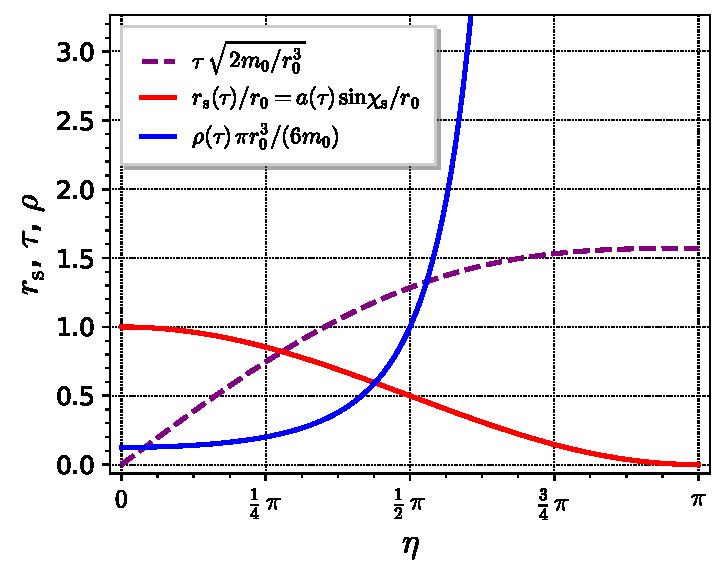
\includegraphics[width=0.48\textwidth]{lem_OS_rs_rho_eta.pdf}\quad
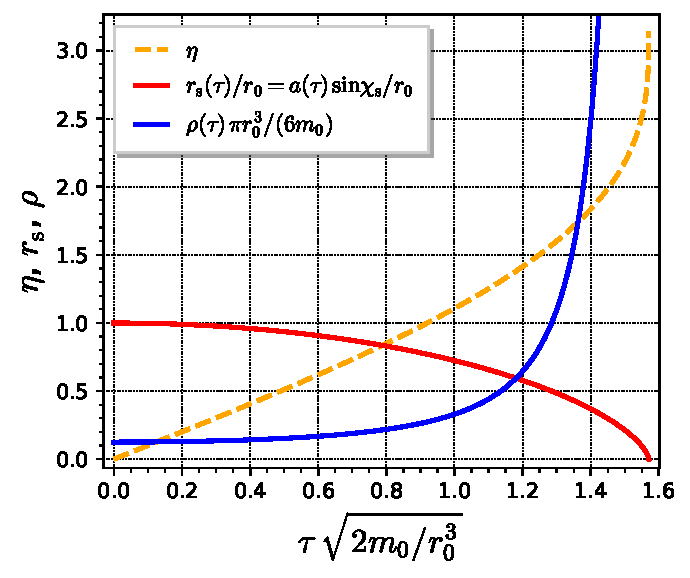
\includegraphics[width=0.45\textwidth]{lem_OS_rs_rho_tau.pdf}
}
\caption[]{\label{f:lem:OS:rs_tho} \footnotesize
Evolution of the areal radius $r_{\rm s}(\tau)$ the collapsing star [Eq.~(\ref{e:lem:OS:evol_star_surf}); red curve] and of the proper matter density
$\rho(\tau)$ [Eq.~(\ref{e:lem:OS:rho_tau}); blue curve] in terms of the conformal time $\eta$ (left)
or the matter proper time $\tau$ (right).  The function $\tau = \tau(\eta)$ is depicted by the purple dashed curve, while its inverse, $\eta = \eta(\tau)$, is depicted by the orange dashed one.
As indicated in the legends, the plot of metric
factor $a(\tau)$ is the same as that of $r_{\rm s}(\tau)$ up to a rescaling
by $\sin\chi_{\rm s}$.
\textsl{[Figures generated by the notebook \ref{s:sam:Oppenheimer_Snyder}]}
}
\end{figure}


The matter density $\rho(\tau,\chi)$ is deduced from Eq.~(\ref{e:lem:LTeqs2}), with the above
values of $M(\chi)$ and $r(\tau,\chi)$. We get a function of $\tau$ only,
via $\eta = \eta(\tau)$ [cf. Eq.~(\ref{e:lem:OS:tau_r_eta})],
which we rewrite as $\rho(\tau)$:
\be \label{e:lem:OS:rho_tau}
  \encadre{  \rho(\tau) = \frac{6 m}{\pi r_0^3 (1 + \cos\eta)^3} } .
\ee
% \rho(\tau) = \frac{3 a_0}{8\pi a(\tau)^3}
The independence of $\rho$ from $\chi$ confirms that the choice
(\ref{e:lem:OS:free_func}) leads to a uniform density object, i.e.
a homogeneous star.
Let us stress that the homogeneity is maintained during all the collapse:
at each instant of matter proper time $\tau$, the density is uniform is all the star.
The function $\rho(\tau)$ is plotted in Fig.~\ref{f:lem:OS:rs_tho}.
\begin{remark}
In view of Eq.~(\ref{e:lem:OS:evol_star_surf}), we may rewrite Eq.~(\ref{e:lem:OS:rho_tau})
as
\be \label{e:lem:OS:rho_m0_r_tau}
    \rho(\tau) = \frac{m}{\frac{4}{3}\pi r_{\rm s}(\tau)^3} .
\ee
This formula happens to be identical to that giving the mass density of a uniform ball of mass
$m$ and radius $r_{\rm s}(\tau)$ in Newtonian physics (flat spacetime), but there is
no profound physical significance in this coincidence.
\end{remark}

It is instructive to express the initial energy density, $\rho_0 := \rho(\tau=0)$,
in terms of the geometrical mass density unit $m^{-2}$ and the compactness
angle $\chi_{\rm s}$ by combining Eqs.~(\ref{e:lem:OS:rho_tau}) and
(\ref{e:lem:OS:sin_chis_m0_r0}):
\be \label{e:lem:OS:rho0}
    \rho_0 = \frac{3 \sin^6\chi_{\rm s}}{32\pi m^2} .
\ee

The metric factor $a(\tau,\chi)$, which appears in Eq.~(\ref{e:lem:metric_sync_coord}),
is deduced from Eq.~(\ref{e:lem:a_f_dr}), with $\dert{r}{\chi}$ computed
from expression (\ref{e:lem:OS:tau_r_eta}); as for $\rho$, we get a function of $\tau$
only, which we rewrite as $a(\tau)$:
\be \label{e:lem:OS:a_tau}
   \encadre{ a(\tau) = \frac{a_0}{2} \left( 1 + \cos\eta \right) }.
\ee
We may then rewrite the second equation in (\ref{e:lem:OS:tau_r_eta}) as
$r(\tau,\chi) = a(\tau) \sin\chi$, so that the metric
tensor (\ref{e:lem:metric_sync_coord}) inside the star takes the form
\be \label{e:lem:OS:g_interior_tau}
  \encadre{ \w{g} = - \dd\tau^2 + a(\tau)^2 \left[ \dd\chi^2
        + \sin^2\chi \left( \dd\th^2 + \sin^2\th\, \dd\ph^2 \right) \right]  } .
\ee
We recognize the \defin{Friedmann-Lemaître-Robertson-Walker (FLRW) metric}\index{Friedmann-Lemaître-Robertson-Walker metric}\index{FLRW metric} corresponding to a closed universe
(cf. e.g. Chap.~3 of Ref.~\cite{PeterU09} or Chap.~17 of Book~3 of Ref.~\cite{DerueU18}).
This is not so surprising since FLRW metrics are solution of Einstein equation based on the hypothesis of homogeneity of constant $\tau$ slices.
We may use $\eta$, instead of $\tau$, as the time coordinate inside the star, thanks to the
relation
\be
    \dd\tau = \frac{a_0}{2} (1 + \cos\eta) \dd\eta ,
\ee
which follows from (\ref{e:lem:OS:tau_r_eta}). We then deduce from Eq.~(\ref{e:lem:OS:g_interior_tau})
that
\be \label{e:lem:OS:g_int}
    \encadre{   \w{g} = \frac{a_0^2}{4} (1 + \cos\eta)^2 \left[ - \dd\eta^2 + \dd\chi^2
        + \sin^2\chi \left( \dd\th^2 + \sin^2\th\, \dd\ph^2 \right) \right] } .
\ee
The term inside square brackets is nothing but the metric $\tilde{\w{g}}$ of the
\emph{Einstein cylinder}\index{Einstein!cylinder} introduced in Sec.~\ref{s:glo:conf_complet_Mink}
[compare Eq.~(\ref{e:glo:tg_Einstein}) with the change of notation $\eta \leftrightarrow \tau$].
Hence, inside the star, the metric $\w{g}$ is conformal to $\w{\tilde{g}}$:
$\w{g} = \Omega^2 \w{\tilde{g}}$,
with the conformal factor $\Omega := a_0/2 (1 + \cos\eta) = a(\tau)$.
For this reason, $\eta$ is called the \defin{conformal time}\index{conformal!time}\index{time!conformal --}.
Note that while $\w{\tilde{g}}$
is a static metric [it obeys Eq.~(\ref{e:sta:static_metric})], $\w{g}$ is not, since
the conformal factor depends on $\eta$.

On each hypersurface $\eta=\mathrm{const}$, or equivalently $\tau = \mathrm{const}$,
the 3-metric $\w{h}$ induced by
the conformal metric $\w{\tilde{g}}$ is the standard metric of the hypersphere\index{hypersphere}
$\mathbb{S}^3$, expressed in terms of the hyperspherical coordinates $(\chi,\th,\ph)$:
\be
    \w{h} = \dd\chi^2 + \sin^2\chi \left( \dd\th^2 + \sin^2\th\, \dd\ph^2 \right) .
\ee
On the whole $\mathbb{S}^3$, $\chi$ ranges from $0$ to $\pi$. Since in the
present case, $\chi \in [0,\chi_{\rm s}]$ with $\chi_{\rm s} < \pi/2$
[Eq.~(\ref{e:lem:OS:range_chi})],
we may view each constant $\eta$ slice of the interior of the collapsing
star as a piece of $\mathbb{S}^3$, scaled by the factor $a(\tau)$
given by Eq.~(\ref{e:lem:OS:a_tau}).
If one uses the conformal coordinates $(\eta,\chi)$ to draw a 2-dimensional
spacetime diagram of the interior, as in the left part of Fig.~\ref{f:lem:OS:diag_int_EF},
then the radial null geodesics appear as straight lines inclined by $\pm 45^\circ$
with the horizontal, reflecting the Minkowskian part $- \dd\eta^2 + \dd\chi^2$
of the metric (\ref{e:lem:OS:g_int}).

To show that the FLRW interior (\ref{e:lem:OS:g_int})
along with the Schwarzschild exterior (\ref{e:lem:OS:exterior_metric})
form a regular spacetime, one shall check that the
\emph{Darmois junction conditions}\index{Darmois junction conditions}
are fulfilled at the interface between the two regions, i.e. on the
timelike hypersurface $\Sigma$ defining the surface of the collapsing star.
These conditions, first enounced by Georges Darmois\index{Darmois, G.} \cite{Darmo1927}
(see also Sec.~21.13 of MTW textbook \cite{MisneTW73}, as well as Ref.~\cite{Lake17}),
are the continuity of the induced 3-metric of $\Sigma$ and of
its extrinsic curvature\index{extrinsic!curvature}\index{curvature!extrinsic},
when these two tensors are computed on each side of $\Sigma$.
These geometric conditions translate the absence of surface layers on $\Sigma$.
We shall not check them here; the computation can be found in
Sec.~3.8 of Poisson's textbook \cite{Poiss04}.


\begin{figure}
\centerline{
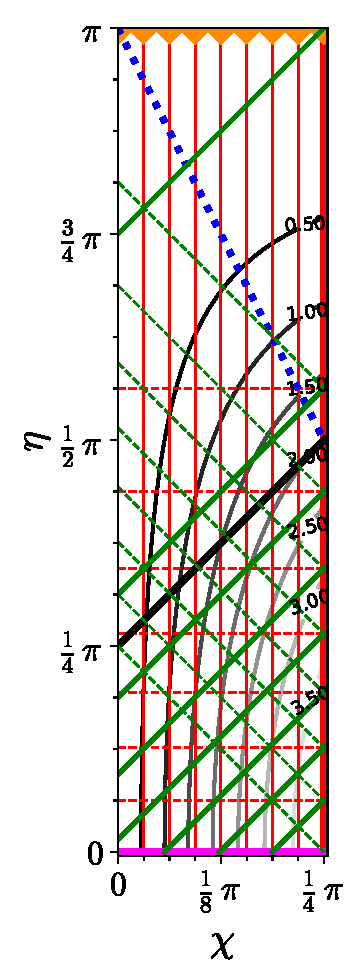
\includegraphics[height=0.55\textheight]{lem_OS_diag_int.pdf}\qquad
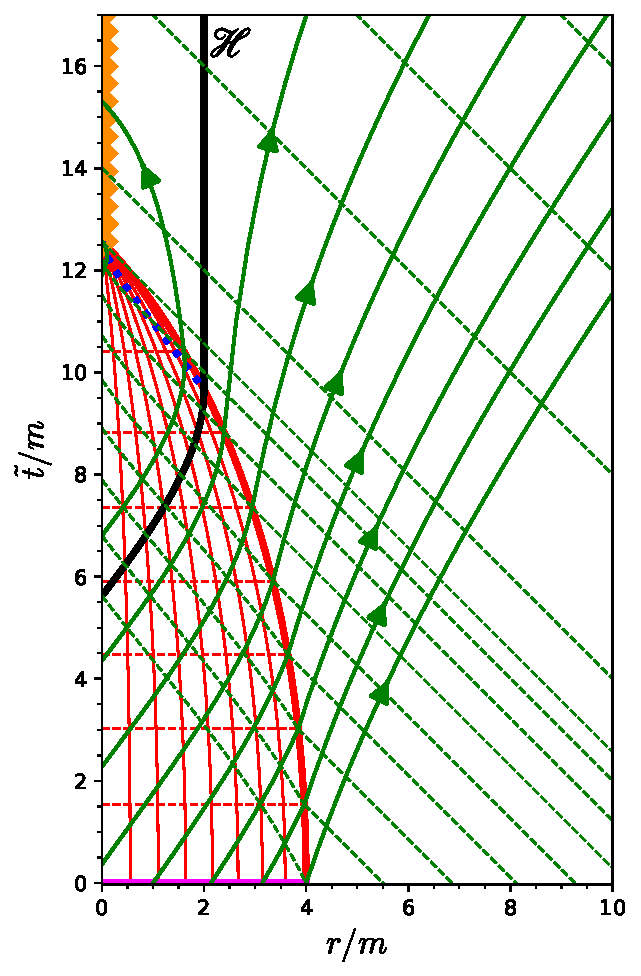
\includegraphics[height=0.6\textheight]{lem_OS_diag_EF.pdf}
}
\caption[]{\label{f:lem:OS:diag_int_EF} \footnotesize
Spacetime diagrams of the Oppenheimer-Snyder collapse
in conformal coordinates $(\eta,\chi)$ (left figure, depicting only the
interior)
and in Eddington-Finkelstein coordinates $(\ti, r)$
(right figure), for the initial compactness $m/r_0 = 1/4$, which corresponds to $\chi_{\rm s} = \pi/4$.
In both figures, solid red lines are worldlines of matter particles,
uniformly sampling $[0,\chi_{\rm s}]$ with $\delta\chi=\pi/32$,
while dashed red lines denote isosurfaces of constant matter proper time $\tau$
uniformly sampling $[0,\tau_{\rm end}]$ with $\delta\tau = \tau_{\rm end}/8$.
The thick red line is the star's surface and the thick magenta one is
the star at the initial instant $\tau=0$. The orange zigzag line marks the
curvature singularity. Solid (resp. dashed) green lines are outgoing (resp. ingoing) radial null geodesics
encountering the star's surface at the above selected values of $\tau$.
The thick black line is the black hole event horizon $\Hor$ and the dotted blue line
is the centered future inner trapping horizon $\mathscr{T}$. In the left figure,
thin solid grey to black lines mark isosurfaces of constant values of the areal radius
$r(\tau,\chi)$ (labeled in units of $m$).
\textsl{[Figures generated by the notebook \ref{s:sam:Oppenheimer_Snyder}]}
}
\end{figure}


\begin{figure}
\centerline{
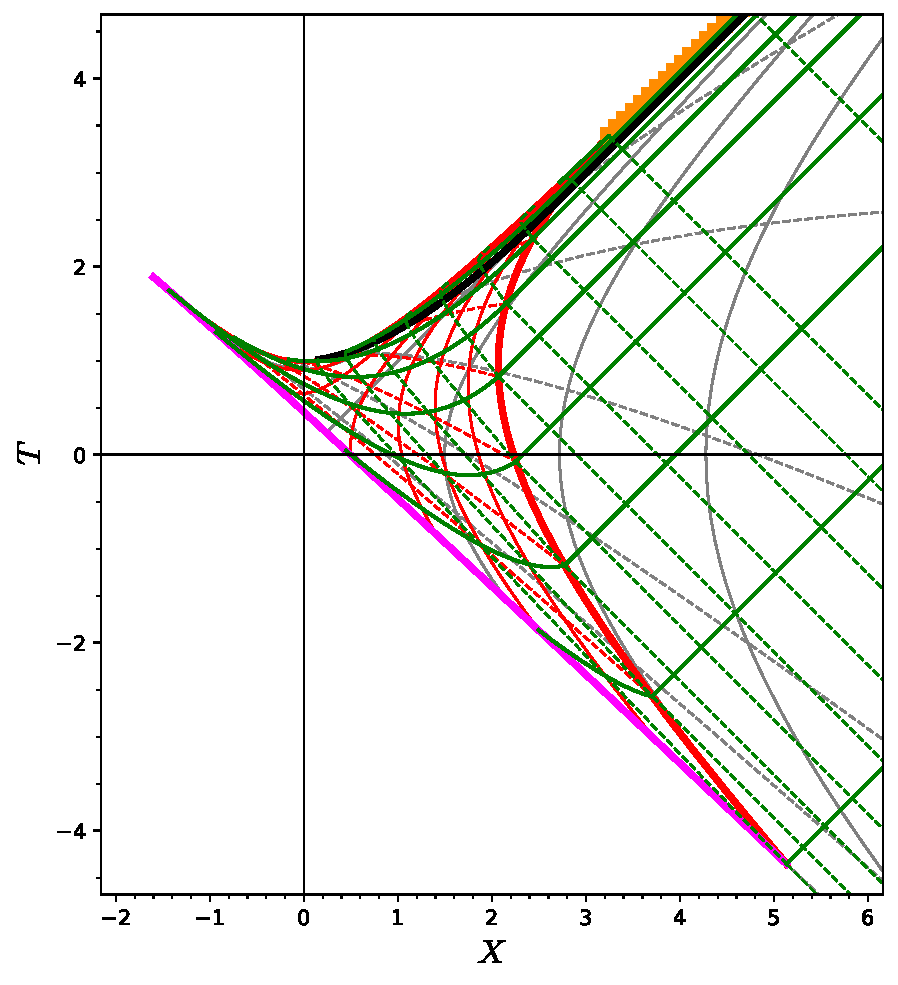
\includegraphics[width=0.55\textwidth]{lem_OS_diag_KS.pdf}\quad
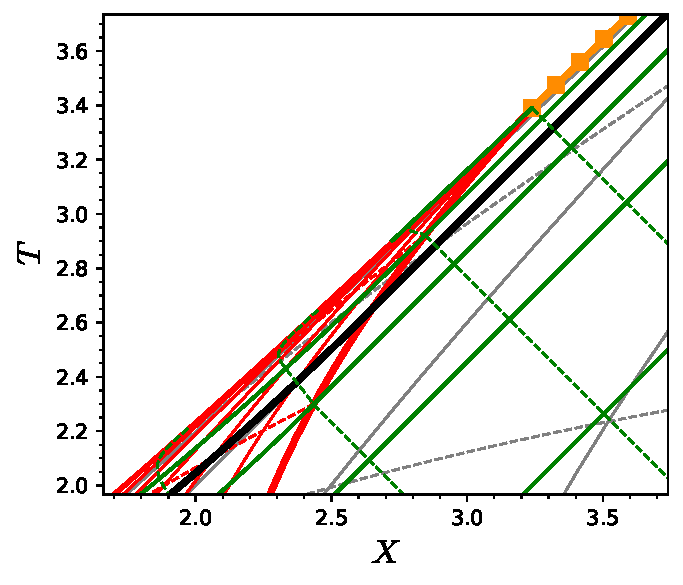
\includegraphics[width=0.45\textwidth]{lem_OS_diag_KS_zoom.pdf}
}
\caption[]{\label{f:lem:OS:diag_KS} \footnotesize
Spacetime diagrams of the Oppenheimer-Snyder collapse
in Kruskal-Szekeres-type coordinates $(T,X)$.
The colored curves are the same as in Fig.~\ref{f:lem:OS:diag_int_EF}.
In particular, the magenta curve represents the star at $\tau = \tilde{t} = 0$,
when the collapse starts. In addition, solid grey
lines are hypersurfaces of constant $r$, uniformly sampling $[0, 8m]$
with $\delta r = m$ and dashed lines are hypersurfaces of
constant $\tilde{t}$, uniformly sampling $[0, 16m]$ with
$\delta\tilde{t} = 2 m$.
The right figure is a zoom on the end of the collapse.
\textsl{[Figures generated by the notebook \ref{s:sam:Oppenheimer_Snyder}]}
}
\end{figure}

\begin{hist}
As mentioned above, the solution originally obtained by J. Robert Oppenheimer\index{Oppenheimer, J.R.}
and Hartland Snyder\index{Snyder, H.S.} in 1939 \cite{OppenS1939}
regards pressureless matter evolving on marginally bound timelike geodesics, i.e. matter
in free fall from $r\to +\infty$, where it is at rest at $\tau\to -\infty$.
More precisely, Oppenheimer and Snyder's original solution corresponds to the choice
\be
    f(\chi) = 1 \qquad
    M(\chi) = m \frac{\chi^3}{\chi_{\rm s}^3}
    \qand \tau_0(\chi) = \sqrt{\frac{2 \chi_{\rm s}^3}{9 m}}
\ee
for the freely specifiable functions determining the solutions of the Lemaître-Tolman system
(cf. Sec.~\ref{s:lem:sol_lambda_zero}), instead of the choice (\ref{e:lem:OS:free_func})
adopted in this chapter. Choosing $f(\chi)=1$ leads to
$E(\chi) = 0$ [cf. Eq.~(\ref{e:lem:E_f_chi})]
and hence to the solution~(\ref{e:lem:sol_E_zero}), instead of (\ref{e:lem:sol_E_neg}).
This solution is still homogeneous, since $\rho$, computed via Eq.~(\ref{e:lem:LTeqs2}),
is a function of $\tau$ only, but it is less adapted
to a star of finite size collapsing from an equilibrium state than the
solution (\ref{e:lem:sol_E_neg}). The latter, which we are using here, has been first presented
by David Beckedorff\index{Beckedorff, D.L.} in 1962 \cite{Becke62} and popularized by
B. Kent Harrison\index{Harrison, B.K.}, Kip Thorne\index{Thorne, K.S.}, Masami Wakano\index{Wakano, M.}
and John Archibald Wheeler\index{Wheeler, J.A.} in their 1965 monograph on gravitational collapse
\cite{HarriTWW65}, as well as by Misner, Thorne and Wheeler in their 1973 textbook \cite{MisneTW73}.
\end{hist}


\subsection{Spacetime diagrams and maximal extensions}

To draw a full spacetime diagram of the collapse, we may extend the ingoing
Eddington-Finkelstein (IEF) coordinates $(\ti,r,\th,\ph)$, used to described the
Schwarzschild exterior of the star to the interior region by demanding
that relation (\ref{e:lem:OS:ti_star_surf}), which a priori links $\ti$
to $\eta$ at the stellar surface, holds everywhere in the interior.
Regarding the IEF coordinate $r$, it is naturally identified with the areal
radius $r(\eta,\chi)$ given by Eq.~(\ref{e:lem:OS:tau_r_eta}).
The resulting spacetime diagram is shown in the right part of Fig.~\ref{f:lem:OS:diag_int_EF}.
In this diagram, only the ingoing radial null geodesics in the exterior appear
as straight lines, as a consequence of the definition of the IEF coordinates
(cf. Sec.~\ref{s:sch:EF_coord}). The slices of constant proper time $\tau$
(dashed red lines) appear as horizontal line segments by virtue of the above
choice for $\ti$ in the interior. In particular, the star at $\tau = 0$
is depicted by a horizontal magenta segment, as in the $(\eta,\chi)$ diagram
on the left of the figure.

Figure~\ref{f:lem:OS:diag_KS} presents another view of the Oppenheimer-Snyder collapse.
It is built on Kruskal-Szekeres-like coordinates
$(T,X)$ (cf. Sec.~\ref{s:max:KS}). These coordinates are defined from the IEF-like ones $(\ti, r)$ via formulas~(\ref{e:sch:KS_IEF}), with $\ti$ being replaced there by $\ti - 5 m$; this
translation in $\ti$ ensures a better representation of the final
stages of the collapse. One may note that the surface of the star (thick solid red line) is initially
tangent to the hypersurface $r=4 m$ (solide grey line), which is the geometrical translation
of the collapse starting from rest. The part of the diagram that lies to the right of the
thick solid red line is identical to a part of the diagram shown in Fig.~\ref{f:sch:IEF_KS}, which
is expected since both represent a piece of Schwarzschild spacetime. A major difference with
the Kruskal-Szekeres diagram of Fig.~\ref{f:sch:IEF_KS} is that the spacetime diagram shown
in Fig.~\ref{f:lem:OS:diag_KS} is not conformal in the stellar interior: the radial null geodesics
are not straight lines inclined by $\pm 45^\circ$. The outgoing ones even run backwards in $T$
in the left part of the diagram, which means that causal relations cannot be simply inferred there.


\begin{figure}
\centerline{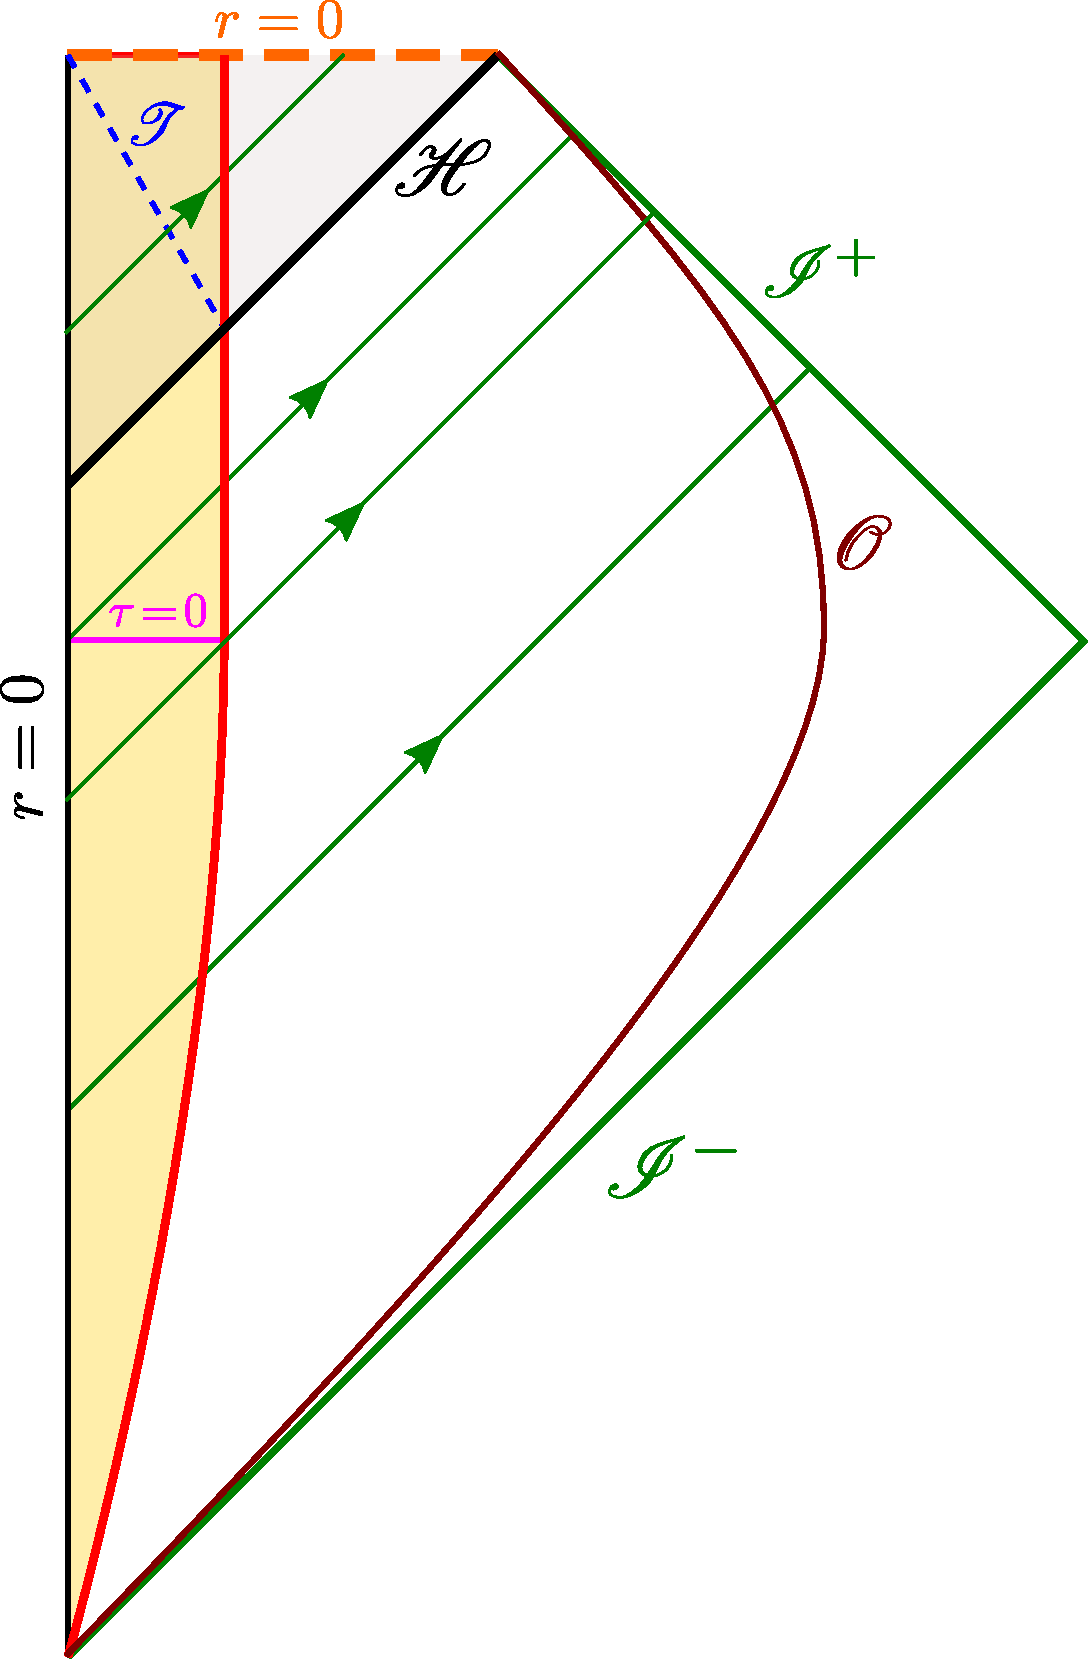
\includegraphics[width=0.4\textwidth]{lem_OS_CP_diag.pdf}}
\caption[]{\label{f:lem:OS:CP_diag} \footnotesize
Carter-Penrose diagram of the Oppenheimer-Snyder collapse generated
by switching off the pressure at $\tau=0$ in a star
in hydrostatic equilibrium for $\tau \in (-\infty,0)$.
The stellar surface is indicated by the red curve and some outgoing radial
null geodesics are drawn as green straight lines.
The black hole event horizon $\Hor$ is indicated by
the black line, the shaded region being the black hole interior.
The dashed blue line marks the trapping horizon
$\mathscr{T}$ discussed in Sec.~\ref{s:lem:trapped},
while the orange zigzag line marks the curvature singularity.
The maroon curve is the worldline of the remote
static observer $\Obs$ considered in Sec.~\ref{s:lem:obs}.
}
\end{figure}

Finally let us consider a compactified conformal diagram of the Oppenheimer-Snyder collapse, i.e.
a \emph{Carter-Penrose diagram}\index{Carter-Penrose diagram}
(cf. Secs.~\ref{s:max:Carter-Penrose} and \ref{s:ker:Carter_Penrose_diag}).
Thanks to the compactification, such a diagram offers a view of the entire spacetime.
It is then natural to consider \emph{maximal} spacetimes,
i.e. spacetimes in which each geodesic is inextendible, being complete or terminating
at a singularity (cf. Sec.~\ref{s:geo:existence_uniqueness}).
This is clearly not the case of the spacetime depicted in the
diagrams of
Figs.~\ref{f:lem:OS:diag_int_EF} and \ref{f:lem:OS:diag_KS}: when run
in the past direction, causal geodesics
in the star interior stop on the hypersurface $\tau=0$
(the magenta line). In particular, the free-falling matter geodesics, along
which $\tau$ is an affine parameter, are clearly incomplete and could a priori
be extended to
$\tau < 0$.

There are actually two ways to maximally extend the Oppenheimer-Snyder spacetime
considered up to now.
The first one corresponds to a star in
hydrostatic equilibrium for $\tau < 0$ and in which the pressure drops suddenly to zero at $\tau = 0$.
This extension is ``astrophysical'' insofar as it models the gravitational collapse of the core of a massive star. Of course the equilibrium for $\tau< 0$ requires
some nonzero pressure inside the star. Therefore it cannot be described by the
Lemaître-Tolman equations discussed in Sec.~\ref{s:lem:LT_equat}; it should rather
obey the \emph{Tolman-Oppenheimer-Volkoff equations}\index{Tolman-Oppenheimer-Volkoff equations},
which govern hydrostatic equilibria in
spherical symmetry (see e.g. Chap.~23 of Ref.~\cite{MisneTW73}).
The Carter-Penrose diagram corresponding to this extension
is drawn schematically (i.e. not by means of explicit coordinates) in Fig.~\ref{f:lem:OS:CP_diag}. The star seems to expand from
the past timelike infinity $i^-$, but this is an artifact of the drawing\footnote{Recall that a
Carter-Penrose diagram reflects the causal structure of spacetime but does not respect the metric distances.}: the star surface
(red line) follows actually a curve $r = \mathrm{const}\; (= r_0)$ for $\tau < 0$. For $\tau \geq 0$,
the surface of the star appears as a vertical line, as in the left part of Fig.~\ref{f:lem:OS:diag_int_EF}, while the radius is actually
decreasing. Actually, one may consider that this
part of the Carter-Penrose diagram is drawn by means of the conformal coordinates $(\eta,\chi)$ used
in Fig.~\ref{f:lem:OS:diag_int_EF}. Note that the Carter-Penrose diagram of Fig.~\ref{f:lem:OS:CP_diag}
corresponds to a maximally extended spacetime: all geodesics are inextendible.
Note as well that the exterior region is formed by parts of regions $\M_{\rm I}$
and $\M_{\rm II}$ of Schwarzschild spacetime (compare with Fig.~\ref{f:max:carter-penrose-std}).

\begin{figure}
\centerline{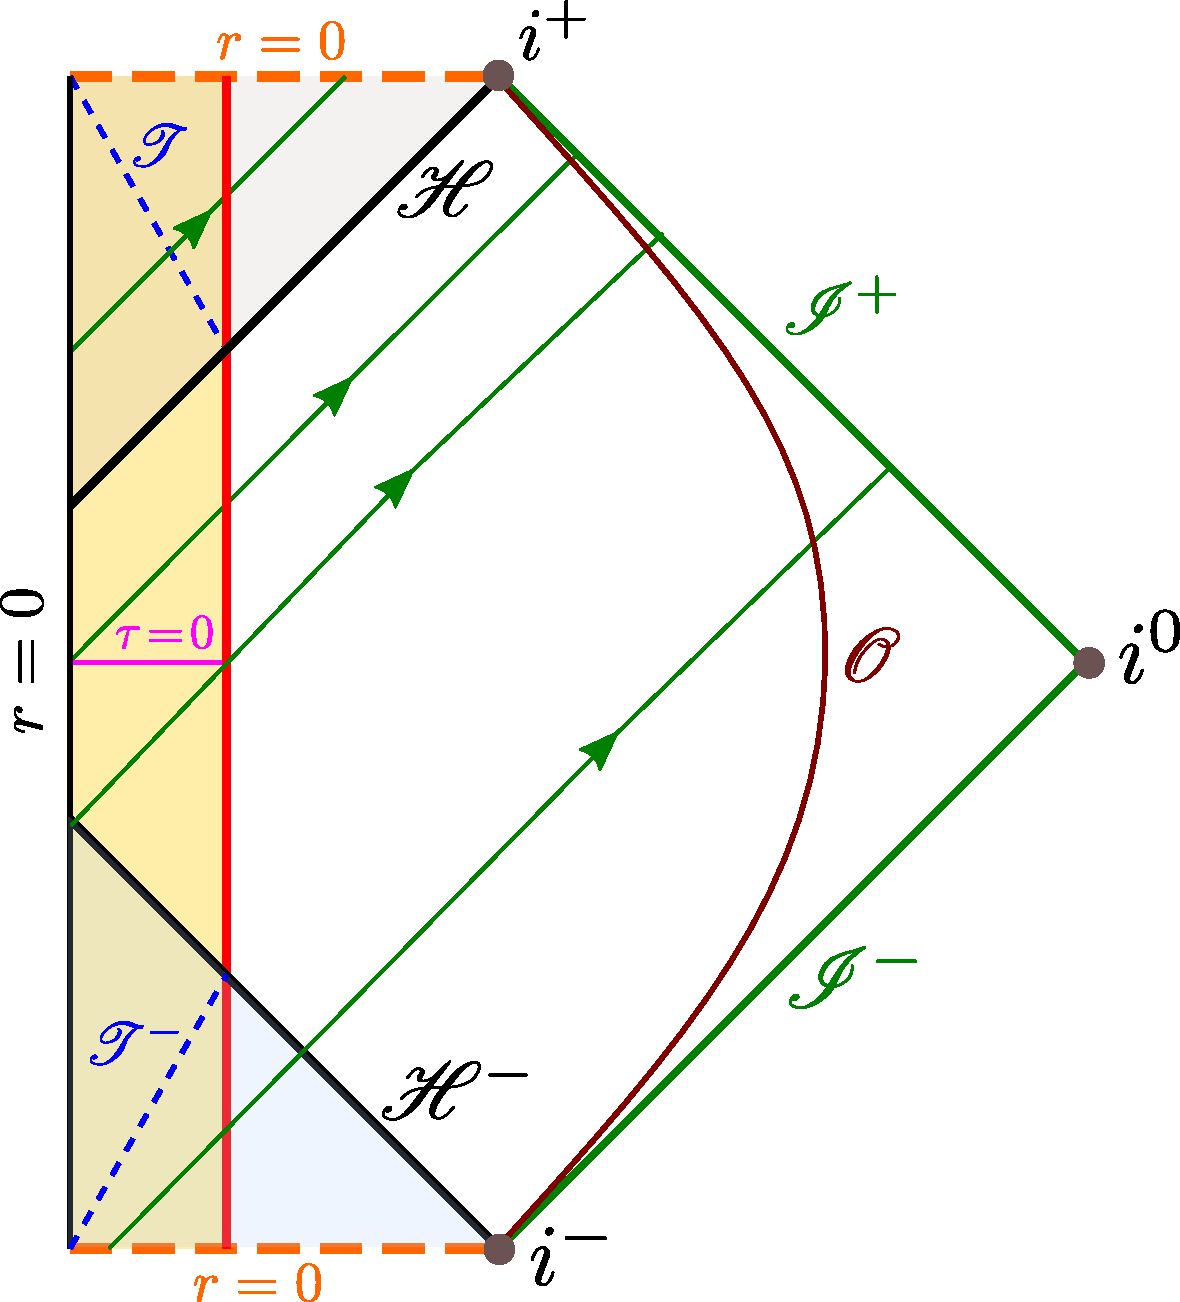
\includegraphics[height=0.35\textheight]{lem_OS_CP_diag_sym.pdf}}
\caption[]{\label{f:lem:OS:CP_diag_sym} \footnotesize
Carter-Penrose diagram of the Oppenheimer-Snyder collapse starting at
the instant of time symmetry ($\tau=0$) after an expanding phase from
a past singularity. The legend is the same as in Fig.~\ref{f:lem:OS:CP_diag},
with in addition the past curvature singularity (bottom orange zigzag line)
and the white hole region (bottom shaded area), bounded by the past event
horizon $\Hor^-$.
}
\end{figure}

The second maximal extension of the Oppenheimer-Snyder spacetime
is based on the assumption that the proper time $\tau=0$ is an instant of
time symmetry of a ball of pressureless matter that was expanding from an
initial past singularity. The spacetime for $\tau < 0$ is then exactly the
time-reversed of that for $\tau > 0$, as illustrated on the Carter-Penrose
diagram of Fig.~\ref{f:lem:OS:CP_diag_sym}.
Such an extension is less ``astrophysical'' than the one considered above, but
it has the advantage to invoke only pressureless matter
and hence to be entirely described by an exact solution of Einstein's equation:
the Friedmann-Lemaître-Robertson-Walker solution (\ref{e:lem:OS:g_int})
extended to $\eta \in (-\pi, \pi)$
inside the star and matched to the Schwarzschild solution
outside the star. This maximal solution contains a \emph{white hole}\index{white hole} region,
i.e. a region in which causal curves arising from the
past null infinity $\scri^-$ cannot penetrate (cf. Sec.~\ref{s:glo:def_BH}).
The white hole (null) boundary is the past event horizon $\Hor^-$ (cf. Fig.~\ref{f:lem:OS:CP_diag_sym}).
The pressureless matter starts its life by expanding from a past curvature singularity where $r=0$,
as a ``mini big-bang'',
the areal radius being given by Eq.~(\ref{e:lem:OS:tau_r_eta}) with $\eta\in (-\pi,0)$
in the expansion phase and $\eta \in (0, \pi)$ in the collapse phase.
Note that the exterior region is formed by parts of regions $\M_{\rm I}$,
$\M_{\rm II}$ and $\M_{\rm IV}$ of the maximally extended
Schwarzschild spacetime (compare with Fig.~\ref{f:max:carter-penrose-std}).
Note also that the star is not visible from the infinite past to the remote static observer
$\Obs$: it only appears to $\Obs$
after the event denoted by $a$ in Fig.~\ref{f:lem:OS:CP_diag_sym}.
On the contrary, in the ``astrophysical'' model discussed above,
the star is always visible to $\Obs$ (cf. Fig.~\ref{f:lem:OS:CP_diag}),
despite it fades very rapidly after the collapse phase has started to be observed,
as we shall see in Sec.~\ref{s:lem:obs}.

\begin{figure}
\centerline{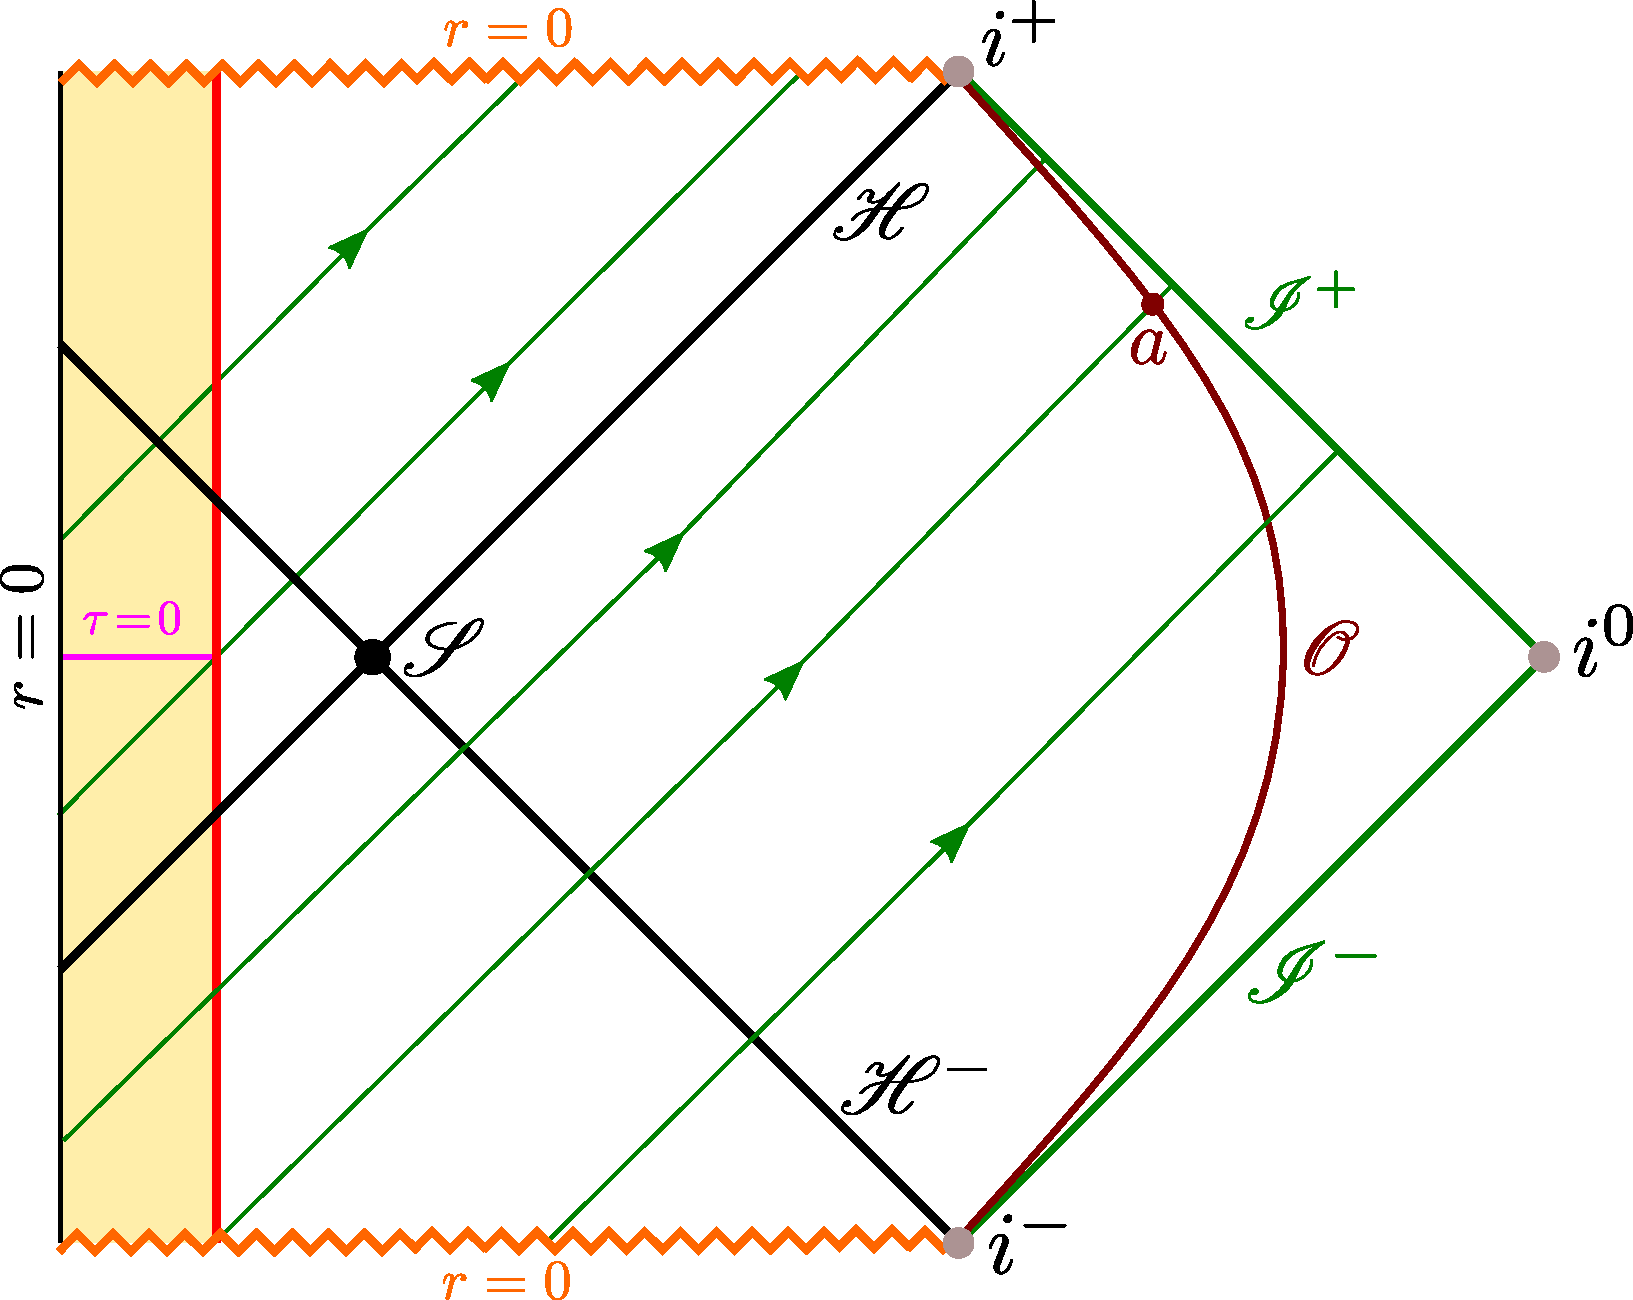
\includegraphics[height=0.35\textheight]{lem_OS_CP_diag_sclosed.pdf}}
\caption[]{\label{f:lem:OS:CP_diag_sclosed} \footnotesize
Carter-Penrose diagram of a semiclosed world. See Fig.~\ref{f:lem:OS:CP_diag_sym}
for the legend.
}
\end{figure}

\begin{remark} \label{r:lem:semiclosed}
The time-symmetric extended solution considered above opens the path
to pressureless solutions with $\chi_{\rm s} \in (\pi/2,\pi)$,
i.e. with $\chi_{\rm s} = \pi - \arcsin\sqrt{2 m/r_0}$ as the solution
of the junction equation (\ref{e:lem:OS:sin_chis_m0_r0}).
We disregarded these solutions in Sec.~\ref{s:lem:OS_sol}, after having noticed
that they lead to the areal radius $r(\tau,\chi)$ being a decreasing function of $\chi$ for
$\chi\in (\pi/2, \chi_{\rm s}]$. In other words, starting from the center of the
star at $\chi = 0$ and keeping $\tau$ fixed, $r(\tau,\chi)$ increases up to the maximum value
$r_{\rm s}(\tau)/\sin\chi_{\rm s}$,
achieved for $\chi=\pi/2$, and then decreases
to $r_{\rm s}(\tau)$ for $\chi = \chi_{\rm s}$. Such a behavior
is possible if the star's surface meets Schwarzschild spacetime in a region
of the latter where $r$ decreases when moving away from the surface (i.e.
``to the right'' if one places the star at the left of a Carter-Penrose diagram
as in Figs.~\ref{f:lem:OS:CP_diag}-\ref{f:lem:OS:CP_diag_sym}).
This happens in the region $\hat{X} < 0$ of the compactified
Kruskal-Szekeres coordinates (cf. Fig.~\ref{f:max:carter-penrose-std}).
We may then place the star there; the corresponding
Carter-Penrose diagram is shown in Fig.~\ref{f:lem:OS:CP_diag_sclosed}.
We note that the star exterior comprises the entire region $\M_{\rm I}$  of
the extended Schwarzschild spacetime, as well as parts of regions $\M_{\rm II}$,
$\M_{\rm III}$ and  $\M_{\rm IV}$. Contrary to the solution
for $\chi_{\rm s} < \pi/2$ shown in Fig.~\ref{f:lem:OS:CP_diag_sym}, it
contains the bifurcation sphere\index{bifurcation!sphere} $\Sp$, where $\Hor$ meets $\Hor^-$
(cf. Sec.~\ref{s:max:bifur_Kill_hor}). Such a configuration is called a \defin{semiclosed world}\index{semiclosed world} (cf. p.~149 of Ref.~\cite{ZeldoN83}, Sec.~2.7 of Ref.~\cite{NovikF89}
or Sec. 2.7.2 of Ref.~\cite{FroloN98}), because at the limit $\chi_{\rm s} \to \pi$, the
matter region becomes an entire FRLW closed universe.
Note that the collapse phase ($\tau > 0$) cannot be seen by a remote static observer, like $\Obs$ in Fig.~\ref{f:lem:OS:CP_diag_sclosed}, for it is hidden below
the event horizon $\Hor$; only some initial part of the expanding phase is visible to $\Obs$
on the segment $a - i^+$ of his worldline.
\end{remark}

\begin{hist}
The \emph{semiclosed world} solutions have been introduced by Oscar Klein\index{Klein, O.}
in 1961 \cite{Klein61} and Yakov B. Zeldovich\index{Zeldovich, Ya.B.} in 1962 \cite{Zeldo62}.
They have been further studied by Igor D. Novikov\index{Novikov, I.D.} in 1963 \cite{Novik63}.
\end{hist}


\subsection{Final singularity}

The collapse ends at $\eta = \pi$, since this value corresponds to the surface
areal radius $r_{\rm s}(\tau) = 0$, by virtue of Eq.~(\ref{e:lem:OS:evol_star_surf}).
Equation~(\ref{e:lem:OS:tau_r_eta}) shows that this corresponds as well
to $r(\tau,\chi) = 0$ for all
particles inside the star. The matter proper time $\tau$ at the end of the collapse
is given by $\eta=\pi$ in Eq.~(\ref{e:lem:OS:tau_r_eta}):
\be \label{e:lem:OS:tau_end}
   \encadre{ \tau_{\rm end} = \frac{\pi}{2} a_0 = \pi \sqrt{\frac{r_0^3}{8 m}}
      = \pi \left( \frac{r_0}{2 m} \right)^{3/2} m
      = \pi \frac{m}{\sin^3\chi_{\rm s}}
      = \sqrt{\frac{3\pi}{32\rho_0}} },
\ee
where the last equality has been obtained by using Eq.~(\ref{e:lem:OS:rho0})
to express $m/\sin^3\chi_{\rm s}$ in terms of the initial proper energy density $\rho_0$.
We note that $\tau_{\rm end}$ is a function of $\rho_0$ only.

\begin{remark}
The above formulas for the collapse proper time $\tau_{\rm end}$ are identical
to those giving the collapse time of a spherical ball of dust of mass $m$, initial radius
$r_0$ and initial mean mass density $\rho_0=3 m/(4\pi r_0^3)$ in Newtonian gravity.
This coincidence arises from the
same cycloidal law for $r_{\rm s}(\tau)$ in both general relativity and Newtonian gravity,
as already discussed in Remark~\ref{r:lem:OS:cycloid} on p.~\pageref{r:lem:OS:cycloid}.
\end{remark}

Similarly, setting $\eta=\pi$ in Eq.~(\ref{e:lem:OS:ti_star_surf}), we get the value
of the IEF coordinate $\ti$ at the end of the collapse:
\be
     \ti_{\rm end} = 2m \left[ \pi \left(1 +  \frac{r_0}{4m} \right) \sqrt{\frac{r_0}{2m} - 1}
     - \ln \left( \frac{r_0}{2m} - 1\right) \right] .
\ee
\begin{example} \label{x:lem:OS:tau_end_plot}
For the compactness $m/r_0 = 1/4$, which is that considered in Figs.~\ref{f:lem:OS:diag_int_EF}-\ref{f:lem:OS:diag_KS}, the above formulas yield
$\tau_{\rm end} = 2 \sqrt{2} \pi m \simeq 8.89\, m$ and
$\ti_{\rm end} = 4 \pi m \simeq 12.57\, m$.
\end{example}

\begin{example} \label{x:lem:OS:tau_end_astro}
Some numerical values of $\tau_{\rm end}$ are given in Table~\ref{t:lem:OS:num} for
various astrophysical objects, if they happen to collapse by a sudden lack
of force acting against gravitation. One sees that the Earth
would collapse in 15 minutes, while it would take half an hour for the Sun,
3 seconds for a white dwarf and a tenth of millisecond for a neutron star.
The similarity of the values for the Earth and the Sun, which have very different
masses and radii, is due to the closeness of their values of $\rho_0$.
\end{example}

\begin{table}
\centerline{
\begin{tabular}{|l|c|c|c|c|}
\hline
& Earth & Sun & white dwarf & neutron star \\[0.5ex]
\hline\hline
$m$ $[M_\odot]$& $3 \; 10^{-6}$ & $1$ & $0.6$ & $1.4$ \\[0.5ex]
\hline
$r_0$ $[{\rm km}]$ & $6.37\; 10^3$ & $6.96\; 10^5$ & $8.0\; 10^3$ &  $12$ \\[0.5ex]
\hline
$m/r_0$ & $7.0\;10^{-10}$ & $2.1\; 10^{-6}$ & $1.1\; 10^{-4}$ & $0.17$ \\[0.5ex]
\hline
$\chi_{\rm s}$ & $3.7\; 10^{-5}$ & $2.1\; 10^{-3}$ & $1.5\; 10^{-2}$ & $0.63$ \\[0.5ex]
\hline
$\rho_0$ $[{\rm kg\, m}^{-3}]$ & $5.5\; 10^3$ & $1.4\; 10^3$ & $5.6\; 10^8$ & $3.8\; 10^{17}$ \\[0.5ex]
\hline
$\tau_{\rm end}$ & $14\; {\rm min}\; 55\; {\rm s}$ & $29\; {\rm min}\; 30\; {\rm s}$ &
$2.82\; {\rm s}$ & $107\; \mu{\rm s}$  \\[0.5ex]
\hline
$\tau_{\rm hb}$ & $14\; {\rm min}\; 55\; {\rm s}$ & $29\; {\rm min}\; 30\; {\rm s}$ &
$2.82\; {\rm s}$ & $75\; \mu{\rm s}$  \\[0.5ex]
\hline
$\tau_{\rm end} - \tau_{\rm hb}$ & $6.7\; 10^{-11}\; {\rm s}$ & $22\; \mu{\rm s}$
& $13\; \mu{\rm s}$ & $32\; \mu{\rm s}$ \\[0.5ex]
\hline
$\tau_{\rm end} - \tau_*$ & $2.0\; 10^{-11}\; {\rm s}$ & $6.6\; \mu{\rm s}$
& $3.9\; \mu{\rm s}$ & $10.4\; \mu{\rm s}$ \\[0.5ex]
\hline
$\rho_{\rm hb}$ $[{\rm kg\, m}^{-3}]$ & $1.8\; 10^{29}$ & $1.8\; 10^{18}$
& $4.5\; 10^{18}$ & $1.4\; 10^{18}$ \\[0.5ex]
\hline
\end{tabular}
}
\caption[]{\label{t:lem:OS:num} \footnotesize
Numerical values for the gravitational collapse of various astrophysical bodies,
assuming that all forces counterbalancing gravitation suddenly disappear
at the proper time $\tau=0$.
$m$ is the gravitational mass (constant during the collapse),
$r_0$ is the initial areal radius, $m/r_0$ is the initial compactness,
$\chi_{\rm s}$ is the (constant) value of the hyperspherical angle $\chi$ at the surface
of the body [Eq.~(\ref{e:lem:OS:chis_m0_r0})], $\rho_0$ is the initial
proper energy density, assuming that the body is homogeneous
[Eq.~(\ref{e:lem:OS:rho_m0_r_tau}) with $\tau=0$, or Eq.~(\ref{e:lem:OS:rho0})],
$\tau_{\rm end}$ is the matter proper time at the end of the collapse, when the
central singularity appears [Eq.~(\ref{e:lem:OS:tau_end})],
$\tau_{\rm hb}$ is the matter proper time when the black hole event horizon
forms at the center
of the body [Eq.~(\ref{e:lem:OS:tau_hb})],
$\tau_*$ is the proper time when the horizon encounters
the infalling surface [Eq.~(\ref{e:lem:OS:tau_star})]
and $\rho_{\rm hb}$ is the proper energy density
at $\tau=\tau_{\rm hb}$ [Eq.~(\ref{e:lem:OS:rho_hb})].
}
\end{table}




Equation~(\ref{e:lem:OS:rho_tau}) with $\eta\to \pi$
immediately yields an infinite proper energy density at the end of the collapse:
\be
    \lim_{\tau\to\tau_{\rm end}} \rho(\tau) = + \infty.
\ee
Since $\rho$ is a measurable quantity (by comoving observers), this signals
some physical singularity.
This corresponds actually to the apparition of a \emph{curvature singularity}
in the part of spacetime covering the interior of the star (cf. the discussion
in Sec.~\ref{s:sch:singularities}).
Indeed, from the interior metric (\ref{e:lem:OS:g_int}), one can
evaluate\footnote{See the notebook \ref{s:sam:Oppenheimer_Snyder_curvature} for
the computations.} curvature scalars like the Ricci scalar
\be \label{e:lem:OS:Ricci_scal}
    R := R^\mu_{\ \, \mu} = \frac{24}{a_0^2 (1 + \cos\eta)^3} = \frac{6 m}{r_{\rm s}(\tau)^3} ,
\ee
the ``square'' of the Ricci tensor
\be \label{e:lem:OS:Ricci_squared}
    R_{\mu\nu} R^{\mu\nu} = \frac{576}{a_0^4 (1 + \cos\eta)^6}
    =  \frac{36 m^2}{r_{\rm s}(\tau)^6}
\ee
and the Kretschmann
scalar\index{Kretschmann scalar! of Oppenheimer-Snyder metric} defined by
Eq.~(\ref{e:sch:def_Kretschmann}):
\be \label{e:lem:OS:Kretschmann}
      K := R_{\mu\nu\rho\sigma} R^{\mu\nu\rho\sigma} = \frac{960}{a_0^4 (1 + \cos\eta)^6}
         = \frac{60 m^2}{r_{\rm s}(\tau)^6} .
\ee
\begin{remark}
Although the components of the Riemann and Ricci tensors with respect to the
coordinates $(\eta,\chi,\th,\ph)$ depend on $\chi$ (cf. the notebook \ref{s:sam:Oppenheimer_Snyder_curvature}),
the above three scalars are independent
of it, in full agreement with the homogeneity of the stellar interior at each
instant $\eta$.
\end{remark}

It is clear that the above three curvature invariants diverge when $\eta\to \pi$,
or equivalently, when $r_{\rm s}(\tau)\to 0$. Hence a curvature singularity
appears in the stellar interior at the end of the collapse.
It is depicted by the orange zigzag segment in left spacetime diagram
of Fig.~\ref{f:lem:OS:diag_int_EF}. This singularity is shrunk to the point
$(\ti, r) = (\ti_{\rm end}, 0)$ in the IEF diagram on the right part of the figure,
because $r_{\rm s}(\tau_{\rm end}) = 0$. It is then connected to the
curvature singularity at $r=0$ of Schwarzschild spacetime, depicted as the
vertical orange zigzag segment.

\begin{remark}
The reader might be puzzled by the Kretschmann scalar (\ref{e:lem:OS:Kretschmann})
being different from that of Schwarzschild spacetime, as given by Eq.~(\ref{e:sch:value_Kretschmann}):
$K_{\rm Schwarz} = 48 m^2/r^6$. Both
have the same $m^2/r^6$ structure but they differ by the numerical prefactor: 60 versus 48.
This actually reflects the discontinuity of the Riemann tensor between the stellar interior
and the Schwarzschild exterior. This discontinuity is enforced on the Ricci part of the Riemann
tensor via the Einstein equation and the uniform density of the star, the latter yielding
a jump of the energy-momentum tensor $\w{T}$ between the value (\ref{e:lem:T_pressureless})
and zero (vacuum exterior). The difference is even more dramatic on the Ricci scalar
(\ref{e:lem:OS:Ricci_scal})
and the square of the Ricci tensor (\ref{e:lem:OS:Ricci_squared}), since they are
identically zero in the Schwarzschild exterior. In other words, the Einstein equation
implies that the metric tensor of the Oppenheimer-Snyder solution is not $C^2$.
For an actual stellar core, there is a density gradient so that $\rho=0$
at the surface and the metric tensor is at least $C^2$.
\end{remark}


\subsection{Black hole formation}

Since the surface areal radius $r_{\rm s}(\tau)$ is a monotonically decreasing function
of $\tau$ (cf. Fig.~\ref{f:lem:OS:rs_tho}), there exists a unique value $\tau_*$ of
$\tau$ for which $r_{\rm s}(\tau_*) = 2 m$. For $\tau>\tau_*$, $r_{\rm s}(\tau) < 2 m$
and the exterior
Schwarzschild spacetime contains a black hole event horizon $\Hor$, located
at $r=2m$ in IEF coordinates (the vertical black segment in Fig.~\ref{f:lem:OS:diag_int_EF}).
The value of $\tau_*$ is determined through the corresponding
conformal time $\eta_*$ via Eq.~(\ref{e:lem:OS:evol_star_surf}):
\[
    \frac{r_0}{2} (1 + \cos\eta_*) = 2 m \iff
    \cos\eta_* = 4\frac{m}{r_0} - 1 = 2 \sin^2\chi_{\rm s} - 1 = - \cos(2\chi_{\rm s}) ,
\]
where use has been made of Eq.~(\ref{e:lem:OS:sin_chis_m0_r0}). Given that $0<\eta_*<\pi$
and $0<\chi_{\rm s} < \pi/2$, the solution is
\be \label{e:lem:OS:eta_star}
    \eta_* = \pi - 2 \chi_{\rm s} .
\ee
Equation~(\ref{e:lem:OS:evol_star_surf}) yields then
\be \label{e:lem:OS:tau_star}
  \encadre{  \tau_* = \frac{\pi - 2 \chi_{\rm s} + \sin(2\chi_{\rm s})}{\sin^3\chi_{\rm s}} m
     =  \left( 1 - \frac{2\chi_{\rm s} - \sin(2\chi_{\rm s})}{\pi} \right) \tau_{\rm end} } .
\ee

\begin{example} \label{x:lem:OS:tau_star_chis4}
For the compactness $1/4$ considered in
Figs.~\ref{f:lem:OS:diag_int_EF}-\ref{f:lem:OS:diag_KS}, one has $\chi_{\rm s}=\pi/4$,
so that $\eta_* = \pi/2$ and
$\tau_* = \sqrt{2}(\pi + 2) m \simeq 7.27 \, m \simeq 0.82 \, \tau_{\rm end}$.
\end{example}

\begin{example} \label{x:lem:OS:tau_star_astro}
Values of $\tau_*$ for the various objects considered in Example~\ref{x:lem:OS:tau_end_astro}
are given in Table~\ref{t:lem:OS:num}. We note that for the collapsing Earth, Sun and white dwarf,
$\tau_*$ is very close to $\tau_{\rm end}$, while for the collapsing neutron star,
$\tau_* \simeq 0.9 \, \tau_{\rm end}$. This reflects the smallness of $\chi_{\rm s}$ for
the first three objects, since Eq.~(\ref{e:lem:OS:tau_star}) implies
$\tau_*/\tau_{\rm end} \simeq 1 - 4 \chi_{\rm s}^3/(3\pi)$ for $\chi_{\rm s} \ll 1$.
\end{example}

For $\tau < \tau_*$, one has $r_{\rm s}(\tau) > 2 m$ and the event horizon
must be located inside the collapsing star. To determine it,
let us consider the outgoing radial null geodesics, which are drawn as solid green curves
in Fig.~\ref{f:lem:OS:diag_int_EF}. In view of the metric (\ref{e:lem:OS:g_int}),
the equation of such a geodesic is very simple in terms of
the coordinates $(\eta,\chi)$: $\eta = \chi - \chi_{\rm s} + \eta_{\rm s}$, where
the constant $\eta_{\rm s}$ is the value of $\eta$ when the geodesic
reaches the surface of the star ($\chi = \chi_{\rm s}$). Radial null geodesics
for which $\eta_{\rm s} < \eta_*$ emerge out of the star in
a part of Schwarzschild spacetime where $r > 2 m$, so that they can espace
to infinity. On the contrary, geodesics having $\eta_{\rm s} > \eta_*$ emerge in the
black hole region of Schwarzschild spacetime; they are thus trapped and
eventually end on the curvature singularity at $r=0$. The event horizon
is generated by the null radial geodesics of the limiting case: $\eta_{\rm s} = \eta_*$.
Hence, inside the star, the equation of the black hole event horizon $\Hor$
is $\eta = \chi - \chi_{\rm s} + \eta_*$. Given the value (\ref{e:lem:OS:eta_star}) for
$\eta_*$, we get
\be \label{e:lem:OS:Hor_eta_chi}
    \Hor:\quad \encadre{ \eta = \chi + \pi - 3 \chi_{\rm s} } .
\ee
For a fixed value of $(\th,\ph)$, this is the equation of a straight line segment
inclined by $+45^\circ$ with
respect to the horizontal (cf. Fig.~\ref{f:lem:OS:diag_int_EF}, left).

The equation of $\Hor$ in terms of the internal IEF coordinate is obtained in parametric
form, with parameter $\chi\in[0,\chi_{\rm s}]$ by substituting (\ref{e:lem:OS:Hor_eta_chi})
for $\eta$ in Eq.~(\ref{e:lem:OS:ti_star_surf}) providing $\ti$ and in
Eq.~(\ref{e:lem:OS:tau_r_eta}) providing $r$. One obtains then a curved segment
in the $(\ti, r)$ plane, which
is drawn in black in Fig.~\ref{f:lem:OS:diag_int_EF}, right.

In view of Eq.~(\ref{e:lem:OS:Hor_eta_chi}), we may state:
\begin{prop}[birth and growth of the event horizon]
\begin{itemize}
\item If $\chi_{\rm s} \leq \pi/3$, or equivalently if $m/r_0 \leq 3/8$,
the event horizon $\Hor$ appears at the center of the star ($\chi=0$)
at the conformal time
\be \label{e:lem:OS:eta_hb}
    \eta_{\rm hb} = \pi - 3 \chi_{\rm s}
\ee
or equivalently at the matter proper time
\be \label{e:lem:OS:tau_hb}
  \tau_{\rm hb} = \frac{\pi - 3 \chi_{\rm s} + \sin(3\chi_{\rm s})}{\sin^3\chi_{\rm s}} m
     =  \left( 1 - \frac{3\chi_{\rm s} - \sin(3\chi_{\rm s})}{\pi} \right) \tau_{\rm end} ,
\ee
the label `hb' standing for ``horizon birth''.
\item If $\chi_{\rm s} > \pi/3$, or equivalently if $m/r_0 > 3/8$, the
event horizon $\Hor$ is already present in the star at $\tau=0$, at the
location $\chi = 3\chi_{\rm s} - \pi$.
\end{itemize}
In all cases, the horizon expands according to Eq.~(\ref{e:lem:OS:Hor_eta_chi}) until it reaches the surface
of the star ($\chi=\chi_{\rm s}$) at $\eta = \eta_* = \pi - 2 \chi_{\rm s}$
or $\tau = \tau_*$ given by Eq.~(\ref{e:lem:OS:tau_star}).
\end{prop}

\begin{example}
Continuing with Example~\ref{x:lem:OS:tau_star_chis4}, i.e. with
$m/r_0=1/4$, or equivalently with $\chi_{\rm s}=\pi/4$,
we get $\eta_{\rm hb} = \pi/4$, which corresponds to the origin of the
black straight segment drawn in Fig.~\ref{f:lem:OS:diag_int_EF}, left.
Equation~(\ref{e:lem:OS:tau_hb}) gives
$\tau_{\rm hb} = (2 + \pi/\sqrt{2}) m \simeq 4.22 \, m \simeq 0.48 \, \tau_{\rm end}$.
\end{example}

\begin{figure}
\centerline{
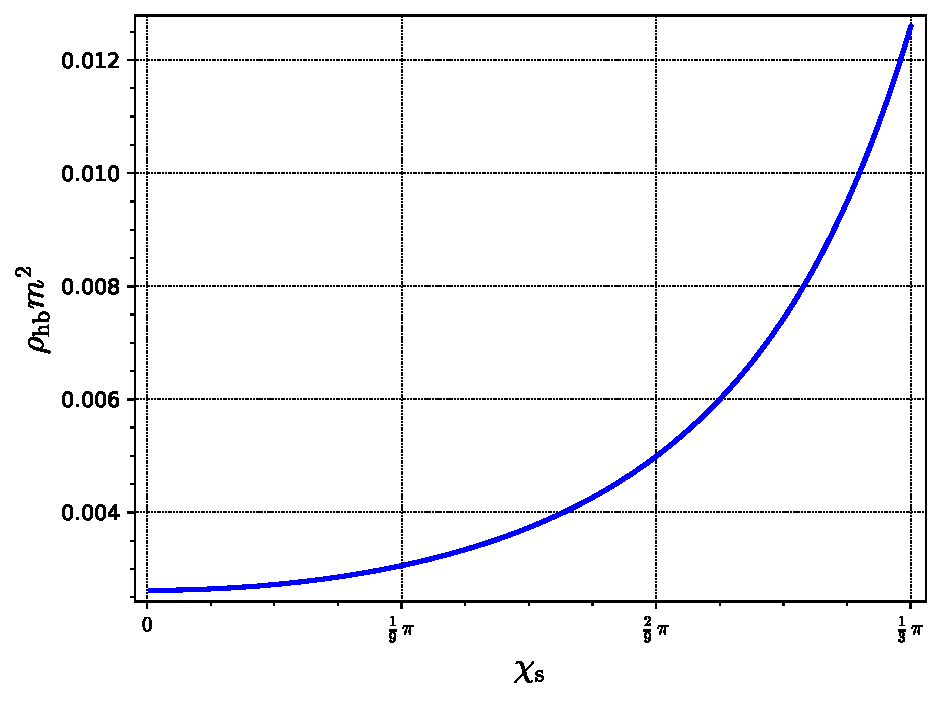
\includegraphics[height=0.35\textheight]{lem_OS_rho_hb.pdf}
}
\caption[]{\label{f:lem:OS:rho_hb} \footnotesize
Proper energy density $\rho_{\rm hb}$ at the instant of the black hole
formation at the center of the star, in units of $m^{-2}$,
as a function of the initial compactness angle $\chi_{\rm s}$.
\textsl{[Figure generated by the notebook \ref{s:sam:Oppenheimer_Snyder}]}
}
\end{figure}

\begin{example} \label{x:lem:OS:tau_hb}
Values of $\tau_{\rm hb}$ for the various objects considered in
Examples~\ref{x:lem:OS:tau_end_astro} and \ref{x:lem:OS:tau_star_astro}
are given in Table~\ref{t:lem:OS:num}. As for $\tau_*$, we note that
for the collapsing Earth, Sun and white dwarf,
$\tau_{\rm hb}$ is very close to $\tau_{\rm end}$. This follows from
$\tau_{\rm hb} / \tau_{\rm end}  \simeq 1 - 9 \chi_{\rm s}^3/(2\pi)$ for $\chi_{\rm s} \ll 1$.
On the contrary, for the collapsing neutron star,
$\tau_{\rm hb} \simeq 0.7 \, \tau_{\rm end}$.
\end{example}


The matter proper energy density at the horizon birth,
i.e. at $\tau = \tau_{\rm hb}$, is obtained by substituting (\ref{e:lem:OS:eta_hb})
for $\eta$ into Eq.~(\ref{e:lem:OS:rho_tau}); using the identity (\ref{e:lem:OS:sin_chis_m0_r0})
to express $m^3/r_0^3$ in terms of $\chi_{\rm s}$, we get
\be \label{e:lem:OS:rho_hb}
    \rho_{\rm hb} := \rho(\tau_{\rm hb}) = \frac{3}{4\pi m^2} \frac{\sin^6\chi_{\rm s}}{(1 - \cos(3\chi_{\rm s}))^3} .
\ee
It is instructive to take the limit of small initial compactness $m/r_0 \ll 1$,
which corresponds to $\chi_{\rm s} \ll 1$ by virtue of relation~(\ref{e:lem:OS:chis_m0_r0}):
\be \label{e:lem:OS:rho_hb_small_compact}
    \rho_{\rm hb}\simeq \frac{2}{243\pi m^2} \left( 1 + \frac{5}{4} \chi_{\rm s}^2 \right)
    + O(\chi_{\rm s}^4) .
\ee
We deduce from Eqs.~(\ref{e:lem:OS:rho_hb})-(\ref{e:lem:OS:rho_hb_small_compact}) that
\be
    \lim_{\chi_{\rm s}\to 0} \rho_{\rm hb} = \frac{2}{243\pi m^2}
    \simeq 2.62\; 10^{-3} m^{-2}
    \quad\mbox{and}\quad
    \lim_{\chi_{\rm s}\to \pi/2}  \rho_{\rm hb} = \frac{3}{4\pi m^2}
    \simeq 0.239\, m^{-2}.
\ee
Between these two limits, $\rho_{\rm hb}$ has a monotonic behavior, as shown in
Fig.~\ref{f:lem:OS:rho_hb}. In particular, we have
\be
    \rho_{\rm hb} < \frac{1}{4 m^2} .
\ee
Hence
\begin{prop}[matter density at the horizon's birth]
By selecting a sufficiently large mass $m$, the matter proper energy density
when the black hole region forms at the center of the collapsing star
can be made arbitrarily small.
\end{prop}
\begin{example} \label{x:lem:OS:rho_hb_water}
Let us determine the mass $m$ for which  $\rho_{\rm hb}$ is as small as
the density of water: $\rho_{\rm hb} = 10^3 \; {\rm kg\, m}^{-3}$.
By restoring the $G$'s and the $c$'s, the density $m^{-2}$ becomes
$c^6/G^3 m^{-2}$.  We then get $m \simeq 4\; 10^7 M_\odot$ for small initial compactness
($\chi_{\rm s} \ll 1$)
and $m \simeq 4\; 10^8 M_\odot$ for large initial compactness
($\chi_{\rm s} \sim \pi/2$).
\end{example}

The relative density increase at the horizon birth with respect to the initial
value $\rho_0 = m/(4/3 \,\pi r_0^3)$ is obtained by setting $\eta = \pi - 3 \chi_{\rm s}$
in Eq.~(\ref{e:lem:OS:rho_tau}):
\be \label{e:lem:OS:rho_hb_rho0}
    \frac{\rho_{\rm hb}}{\rho_0} = \frac{8}{(1 - \cos(3\chi_{\rm s}))^3} .
\ee
For small compactness, we get
\be \label{e:lem:OS:rho_hb_rho0_small_chis}
    \frac{\rho_{\rm hb}}{\rho_0} \underset{\chi_{\rm s}\to 0}{\sim} \frac{64}{729 \chi_{\rm s}^6} .
\ee
Hence $\rho_{\rm hb}/\rho_0$ is diverging very rapidly when $\chi_{\rm s}\to 0$.
On the contrary, for $\chi_{\rm s}$ large, $\rho_{\rm hb}/\rho_0$ can be moderate.
Even, for $\chi_{\rm s} = \pi/3$, Eq.~(\ref{e:lem:OS:rho_hb_rho0})
leads to $\rho_{\rm hb}/\rho_0 = 1$, in
agreement with $\tau_{\rm hb} = 0$ for that value of $\chi_{\rm s}$.

\begin{example}
Values of $\rho_{\rm hb}$ for the various objects considered in
Examples~\ref{x:lem:OS:tau_end_astro}, \ref{x:lem:OS:tau_star_astro}
and \ref{x:lem:OS:tau_hb}
are given in Table~\ref{t:lem:OS:num}. These values are all
larger than the nuclear density $\rho_{\rm nuc} = 2\; 10^{17} \; {\rm kg\, m}^{-3}$.
For the Earth, $\rho_{\rm hb}$ is even $\sim 10^{12} \rho_{\rm nuc}$,
in agreement with the diverging behavior (\ref{e:lem:OS:rho_hb_rho0_small_chis}).
On the contrary, for the neutron star, for which $\chi_{\rm s} = 0.63$,
we have only $\rho_{\rm hb} / \rho_0 \simeq 3.7$. By comparing with
Example~\ref{x:lem:OS:rho_hb_water},
we note that all the examples
considered in Table~\ref{t:lem:OS:num} have a mass much smaller to that
required for a low value of $\rho_{\rm hb}$.
\end{example}

\begin{figure}
\centerline{
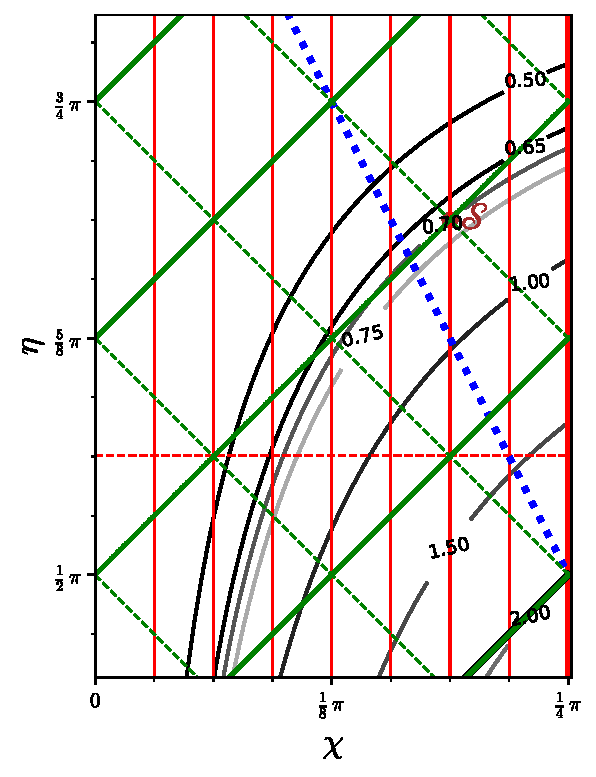
\includegraphics[width=0.45\textwidth]{lem_OS_diag_int_zoom.pdf}\qquad
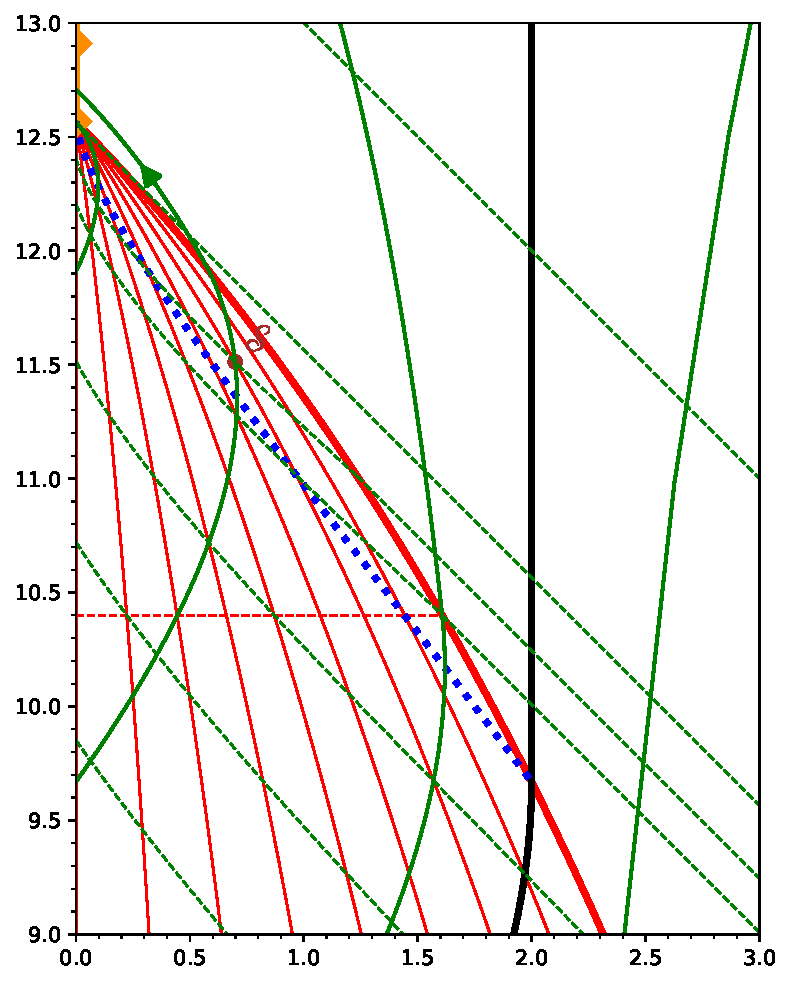
\includegraphics[width=0.5\textwidth]{lem_OS_diag_EF_zoom.pdf}
}
\caption[]{\label{f:lem:OS:diag_trapped} \footnotesize
Spacetime diagrams of the Oppenheimer-Snyder collapse, as in Fig.~\ref{f:lem:OS:diag_int_EF},
but zooming around the trapped sphere $\Sp$ located at $(\eta,\chi) = (11\pi/16, 3\pi/16)$.
The left diagram is drawn in terms of the
conformal coordinates $(\eta,\chi)$, while the right one is based on
the Eddington-Finkelstein coordinates $(\ti, r)$.
See the legend of Fig.~\ref{f:lem:OS:diag_int_EF} for the meaning of the
various curves.
\textsl{[Figures generated by the notebook \ref{s:sam:Oppenheimer_Snyder}]}
}
\end{figure}




\subsection{Trapped surfaces} \label{s:lem:trapped}

The concept of trapped surface\index{trapped!surface}
has been introduced in Sec.~\ref{s:neh:trapped_surfaces}
(cf. Fig.~\ref{f:neh:trapped_surf}).
Let us show that such surfaces appear at late times in the Oppenheimer-Snyder collapse.
To this aim, we consider a 2-dimensional surface $\Sp$ at constant coordinates $(\eta,\chi)$
inside the collapsing star, with $\eta\neq \pi$ and $\chi\neq 0$.
Such a surface appears as a point in the spacetime diagrams of
Fig.~\ref{f:lem:OS:diag_trapped}. The surface $\Sp$
has the topology of a 2-sphere and
is spanned by the coordinates $(\th,\ph)$. In particular,
it is a \emph{closed} manifold (compact
without boundary).
The metric $\w{q}$ induced by $\w{g}$ on $\Sp$ is readily
obtained by setting $\dd\eta = 0$ and $\dd\chi = 0$ in Eq.~(\ref{e:lem:OS:g_int}):
\be \label{e:lem:OS:metric_q_Sp}
      \w{q} = \frac{a_0^2}{4} (1 + \cos\eta)^2
        \sin^2\chi \left( \dd\th^2 + \sin^2\th\, \dd\ph^2 \right)   .
\ee
This is clearly a Riemannian metric, i.e. $\Sp$ is a spacelike 2-surface
of $(\M,\w{g})$.
At each point of $\Sp$, there are two null directions orthogonal to $\Sp$:
the outgoing one, represented by a solid green line in Fig.~\ref{f:lem:OS:diag_trapped}
and the ingoing one, represented by a dashed green line (see also
Fig.~\ref{f:def:TS_ortho}). Future-directed null vectors along these
two directions are respectively
\be \label{e:lem:OS:comp_l_k}
    \wl = \wpar_\eta + \wpar_\chi \qand
    \w{k} = \wpar_\eta - \wpar_\chi .
\ee
The expansions of $\Sp$ along $\wl$ and $\w{k}$ are
given by Eq.~(\ref{e:def:theta_deps_ln_q}) [see also Eq.~(\ref{e:neh:expansion_k})
and Fig.~\ref{f:neh:trapped_surf}]:
\be
     \theta_{(\wl)} = \Lie{\el} \ln \sqrt{q}
     \qand
     \theta_{(\w{k})} = \Lie{\w{k}}  \ln \sqrt{q} ,
\ee
where $q$ is the determinant of the metric $\w{q}$ with respect to any
coordinate system of $\Sp$ that is carried along with $\wl$ or $\w{k}$,
such that $(\th,\ph)$, since $\th$ and $\ph$ are constant along the integral
curves of $\wl$ and $\w{k}$ (the radial null geodesics). From Eq.~(\ref{e:lem:OS:metric_q_Sp}),
we get $\sqrt{q}= (a_0^2/4)(1 + \cos\eta)^2 \sin^2\chi \sin\th$.
Furthermore, in view of the components (\ref{e:lem:OS:comp_l_k}),
$\Lie{\wl} \ln \sqrt{q} = \ell^\mu \partial \ln \sqrt{q} /\partial x^\mu =
 \partial \ln \sqrt{q} /\partial \eta + \partial \ln\sqrt{q} /\partial \chi$
 and
 $\Lie{\w{k}} \ln \sqrt{q} = k^\mu \partial \ln\sqrt{q} /\partial x^\mu =
 \partial \ln\sqrt{q} /\partial \eta - \partial\ln  \sqrt{q} /\partial \chi$.
We then get easily
\be
    \theta_{(\wl)} = 4 \frac{\cos\left(\eta/2\right) \cos\left(\chi + \eta/2\right) }{
    (1 + \cos\eta)\sin\chi}
    \qand
    \theta_{(\w{k})} = - 4 \frac{\cos\left(\eta/2\right) \cos\left(\chi - \eta/2\right) }{
    (1 + \cos\eta)\sin\chi} .
\ee
Given that $\eta\in [0,\pi)$ %]$
and $\chi\in(0,\chi_{\rm s}]$, with $\chi_{\rm s} < \pi/2$,
one has $1 + \cos\eta > 0$, $\cos(\eta/2) > 0$, $\sin\chi > 0$
and $\cos(\chi - \eta/2) > 0$. It follows immediately that
\be
    \theta_{(\w{k})} < 0
\ee
and the sign of $\theta_{(\wl)}$ is that of $\cos(\chi + \eta/2)$.
Given that the above ranges of $\eta$ and $\chi$ imply $0 < \chi + \eta/2 < \pi$,
we have $\theta_{(\wl)} < 0 \iff \chi + \eta/2 > \pi/2$, i.e.
\be \label{e:lem:theta_l_neg}
    \theta_{(\wl)} < 0 \iff \eta > \pi - 2 \chi .
\ee
Since $\Sp$ is a closed spacelike 2-surface,
we conclude, in view of the definitions given in Sec.~\ref{s:neh:trapped_surfaces}:
\begin{prop}[trapped surfaces]
At late times, i.e. for $\eta > \pi - 2 \chi$, the spheres $\Sp$ defined
by $(\eta,\chi) = \mathrm{const}$, with $\eta<\pi$ and $\chi>0$,
are trapped surfaces ($\theta_{(\wl)} < 0$ and $\theta_{(\w{k})} < 0$).
These spheres are marginally trapped
($\theta_{(\wl)} = 0$ and $\theta_{(\w{k})} < 0$)
for $\eta = \pi - 2 \chi$
and untrapped ($\theta_{(\wl)} > 0$ and $\theta_{(\w{k})} < 0$) for $\eta <  \pi - 2 \chi$.
\end{prop}

\begin{example}
The trapped surface $\Sp$ corresponding to $(\eta,\chi) = (11\pi/16, 3\pi/16)$
in the Oppen\-heimer-Snyder collapse with $r_0 = 4 m$
is plotted as a brown dot in Fig.~\ref{f:lem:OS:diag_trapped}. According
to Eq.~(\ref{e:lem:OS:tau_r_eta}), the areal radius of $\Sp$ is
$r_{\Sp} = 2\sqrt{2} \sin(3\pi/16) (1 + \cos(11\pi/16)) \simeq 0.70\, m$.
The trapped character of $\Sp$ can be read on Fig.~\ref{f:lem:OS:diag_trapped}:
moving to the future along either the ingoing radial null geodesic (dashed green line)
or the outgoing one (solid green line) leads to spheres of smaller areal radius,
and hence smaller area. This is clear on the left diagram when noticing
that both geodesics encounter the curve $r=0.65\, m$ in the immediate future of $\Sp$.
It is even more immediate on the right diagram since $r$ is read directly on the $x$-axis.
\end{example}

The set formed by all the marginally trapped spheres
of fixed $(\eta,\chi)$
is the hypersurface $\mathscr{T}$ defined by $\theta_{(\wl)} = 0$.
Its equation is obtained by saturating the inequalities
in Eq.~(\ref{e:lem:theta_l_neg}):
\be \label{e:lem:OS:def_T}
    \mathscr{T}:\qquad \eta = \pi - 2\chi.
\ee
As we shall see in
Chap.~\ref{s:loc}, $\mathscr{T}$ is called a
\defin{future inner trapping horizon}\index{future!inner trapping horizon}\index{trapping horizon!future!inner --}.
It is drawn as a dotted blue line in Figs.~\ref{f:lem:OS:diag_int_EF}
and \ref{f:lem:OS:diag_trapped}. Since the slope of that line is $-2$ and
$(\eta,\chi)$ are conformal coordinates, it is clear from the left diagrams
in these figures that $\mathscr{T}$ is a timelike hypersurface. This is
actually a generic feature of future inner trapping horizons, as we shall
see in Chap.~\ref{s:loc}. We note from Figs.~\ref{f:lem:OS:diag_int_EF}
and \ref{f:lem:OS:diag_trapped} that $\mathscr{T}$ forms at the surface of the
collapsing star at the very same instant where the event horizon $\Hor$
reaches the surface.
Indeed, searching for the intersection $\Hor\cap\mathscr{T}$ from the equations
defining the hypersurfaces $\Hor$ and $\mathscr{T}$, i.e. Eqs.~(\ref{e:lem:OS:Hor_eta_chi})
and (\ref{e:lem:OS:def_T}), we get
$(\eta,\chi) = (\pi - 2\chi_{\rm s}, \chi_{\rm s})$, which is the 2-sphere
representing the surface of the collapsing star at $\eta=\pi - 2 \chi_{\rm s}$.

The trapped surfaces $\Sp$ are located ``above'' $\mathscr{T}$, i.e. at
$\eta > \pi - 2 \chi$. The region containing trapped 2-spheres with $r=\mathrm{const}$ actually extend through the collapsing star's surface up to the event horizon $\Hor$. Indeed, the spacetime there
is a piece of the region $\M_{\rm II}$ of Schwarzschild spacetime (cf. Sec.~\ref{s:sch:SD_domain}),
where every 2-sphere at $\ti = \mathrm{const}$ and $r=\mathrm{const}$ is trapped (this is obvious
since both ingoing and outgoing radial null geodesics have decreasing areal radius $r$
towards the future in $\M_{\rm II}$, cf. Fig.~\ref{f:sch:rad_null_geod_EF}).
Outside $\Hor$, i.e. in the $\M_{\rm I}$ region of Schwarzschild spacetime, there is no trapped
surface.

\begin{remark}
The trapping horizon $\mathscr{T}$ is not the boundary of the region where there
exist trapped surfaces
in the Oppenheimer-Snyder collapse, but only the boundary for trapped 2-spheres $\Sp$
centered around $\chi=0$.
Indeed, since the collapsing stellar interior
is homogeneous, the trapped 2-spheres $\Sp$ can
be translated in $\chi$ at fixed $\eta$, leading to other trapped surfaces.
One can then show that such ``translated'' trapped 2-spheres exist in all the region
$\eta > \pi - \chi_{\rm s} - \chi$, which extends to the past of $\mathscr{T}$,
since for $\chi\in[0, \chi_{\rm s})$,  %]$
$ \pi - \chi_{\rm s} - \chi < \pi - 2\chi$.
Furthermore, there exist more complicated trapped surfaces even below
this limit, see Ref.~\cite{BengtJS13} for details.
\end{remark}


%%%%%%%%%%%%%%%%%%%%%%%%%%%%%%%%%%%%%%%%%%%%%%%%%%%%%%%%%%%%%%%%%%%%%%%%%%%%%%%


\section{Observing the black hole formation} \label{s:lem:obs}

Let us consider a remote static observer $\Obs$ who receives electromagnetic
radiation from the surface of a spherically symmetric collapsing star. By
\emph{static}\index{static!observer!in Schwarzschild!spacetime}, it is meant
that the worldline of $\Obs$ is a field line of the static Killing vector
$\w{\xi} = \wpar_t = \wpar_{\ti}$ in the exterior Schwarzschild region
[cf. Eq.~(\ref{e:ges:u_Obs_xi})]. In particular, $\Obs$ evolves at a fixed
value of $(r_\Obs,\th_\Obs,\ph_\Obs)$ of the coordinates $(r,\th,\ph)$
(cf. Fig.~\ref{f:lem:OS:diag_delay}; see also Figs.~\ref{f:lem:OS:CP_diag}
and \ref{f:lem:OS:CP_diag_sym}).
Without any loss of generality,
we choose $\th_\Obs = \pi/2$ and $\ph_\Obs = 0$.
Furthermore, we assume that $\Obs$ is \emph{remote}: $r_\Obs \gg m$.

\begin{figure}
\centerline{
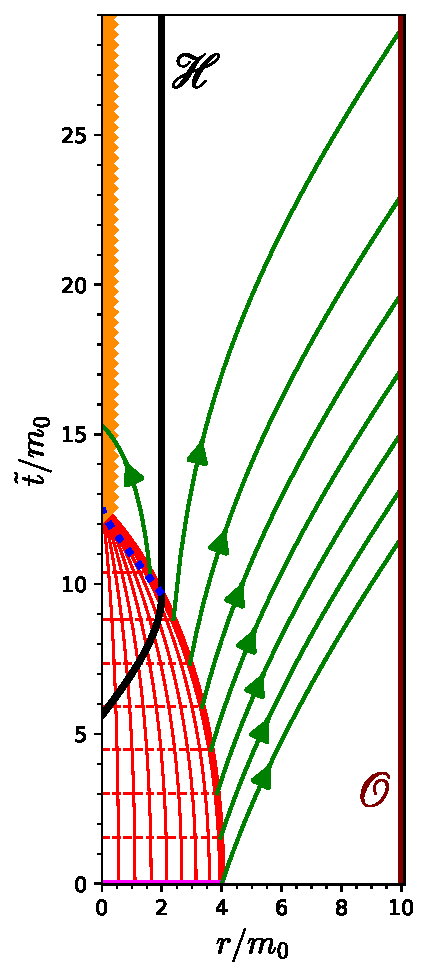
\includegraphics[width=0.3\textwidth]{lem_OS_diag_delay.pdf}
}
\caption[]{\label{f:lem:OS:diag_delay} \footnotesize
Spacetime diagram of the Oppenheimer-Snyder collapse,
as in the right panel of Fig.~\ref{f:lem:OS:diag_int_EF}, illustrating
the increasing delay in the reception by a remote static observer $\Obs$
(maroon worldline at $r=10 \, m$)
of signals emitted radially from the
surface of the collapsing star with a constant interval of matter proper time,
$\delta\tau = \tau_{\rm end}/8$.
See the caption of Fig.~\ref{f:lem:OS:diag_int_EF} for the legend of the various
curves.
\textsl{[Figure generated by the notebook \ref{s:sam:Oppenheimer_Snyder}]}
}
\end{figure}

\subsection{Apparent collapse freezing} \label{s:lem:freezing}

Let us suppose that, at the matter comoving proper time $\tau_1$, an electromagnetic
signal (``flash'') is emitted in the radial direction from
the surface of the collapsing star at $\th=\pi/2$ and $\ph=0$ (i.e. towards observer $\Obs$)
and that a similar signal is emitted
subsequently at proper time $\tau_2$.
Since each signal is carried by an outgoing radial null geodesic (the green curves
in Fig.~\ref{f:lem:OS:diag_delay}), the equation of which is (\ref{e:sch:outgoing_null_geod_EF})
with respect to the IEF coordinates, we have
\[
    \ti^{\rm rec}_i - r_{\Obs} - 4 m \ln \left( \frac{r_{\Obs}}{2 m} - 1 \right) =
    \ti^{\rm em}(\tau_i) - r_{\rm s}(\tau_i) - 4 m \ln \left( \frac{r_{\rm s}(\tau_i)}{2 m} - 1 \right),
    \quad i\in\{1,2\} ,
\]
where $\ti^{\rm rec}_i$ is the IEF coordinate $\ti$ of the reception event of signal no. $i$
by observer $\Obs$ and
$\ti^{\rm em}(\tau_i)$ is the IEF coordinate $\ti$ of the emission event taking place at
proper time $\tau_i$;  $\ti^{\rm em}(\tau_i)$ is given by Eq.~(\ref{e:lem:OS:ti_star_surf})
with $\eta$ being the function of $\tau_i$ defined implicitly by Eq.~(\ref{e:lem:OS:evol_star_surf}).
We deduce from the above relation the $\ti$-interval
separating the receptions of signal 1 and 2 by $\Obs$:
\be \label{e:lem:OS:delay}
    \ti^{\rm rec}_2 - \ti^{\rm rec}_1 =
    \ti^{\rm em}(\tau_2) - \ti^{\rm em}(\tau_1)
    + r_{\rm s}(\tau_1) - r_{\rm s}(\tau_2)
    + 4 m \ln \left( \frac{r_{\rm s}(\tau_1) - 2 m}{r_{\rm s}(\tau_2) - 2 m} \right) .
\ee
Since $\Obs$ is remote ($r_\Obs \gg m$), $\ti^{\rm rec}_2 - \ti^{\rm rec}_1$
is nothing but the lapse of $\Obs$'s proper time between the two reception events.
The quantities $\ti^{\rm em}(\tau_2) - \ti^{\rm em}(\tau_1)$ and $r_{\rm s}(\tau_1) - r_{\rm s}(\tau_2)$
are always finite; on the other side, the logarithm term diverges
when $r_{\rm s}(\tau_2)$ approaches $2 m$, i.e.
when $\tau_2$ approaches $\tau_*$ [cf. Eq.~(\ref{e:lem:OS:tau_star})], so that
\be
    \ti^{\rm rec}_2 - \ti^{\rm rec}_1 \to +\infty
    \quad\mbox{when}\quad \tau_2 \to \tau_* .
\ee
In particular, if a sequence of signals is emitted from the star's surface at a constant rate in terms
of the comoving proper time $\tau$, the signals are received by the remote observer $\Obs$ with an increasing delay as the collapse
proceeds. The delay between two successive signals becoming infinite, there exists a very
last signal received by $\Obs$.
All subsequent signals of the emitted sequence do not cross the event horizon,
i.e. are captured into the black hole.

\begin{example}
Consider Fig.~\ref{f:lem:OS:diag_delay}, which depicts the Oppenheimer-Snyder collapse
with $r_0 = 4 m$, or equivalently $\chi_{\rm s} = \pi/4$. Starting from $\tau=0$, a uniform sequence of 8 signals is emitted from the star's surface, the proper time separation between two successive signals being
$\delta\tau = \tau_{\rm end}/8 = \pi\sqrt{2} m / 4$ (cf. Example~\ref{x:lem:OS:tau_end_plot} on
p.~\pageref{x:lem:OS:tau_end_plot}). One sees graphically that the signals are received by $\Obs$
with an increasing separation $\delta\ti$. The last received signal is the 7th one. The 8th signal is trapped in the black hole region and ends on the curvature singularity.
\end{example}

We conclude from the above analysis:
\begin{prop}[apparent freeze of the collapse]
For a remote static observer, the collapse, as monitored by the reception of signals regularily emitted from the star's surface,
appears to slow down and even to freeze completely when the areal radius
of the star tends towards $2 m$. In particular, the remote observer never sees the
star's surface crossing the event horizon and does not perceive at all the final singularity.
\end{prop}

\begin{hist}
The above behavior explains why the name \emph{frozen star}\index{frozen star}
was given to black holes before the name \emph{black hole} itself was coined
(cf. the historical note on p.~\pageref{h:glo:black_hole_name}).
\end{hist}


\begin{figure}
\centerline{
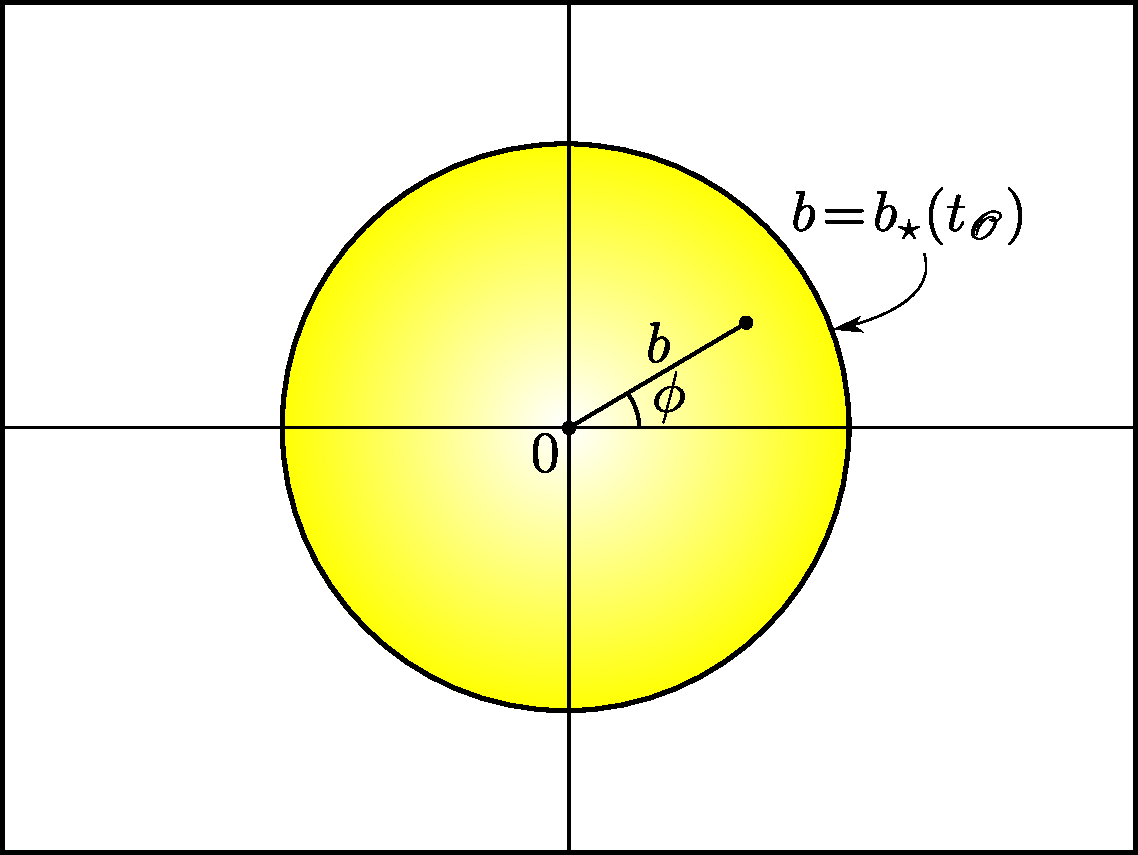
\includegraphics[width=0.5\textwidth]{lem_image.pdf}
}
\caption[]{\label{f:lem:image} \footnotesize
Image of the collapsing star on the screen of the remote observer $\Obs$, at
a given instant $t_\Obs$.
}
\end{figure}


\subsection{Shape and size of the images of the collapse} \label{s:lem:size_image}

The image of the collapsing star is formed on the screen of observer's $\Obs$
by photons emitted from the star's surface and following
null geodesics of Schwarzschild spacetime (the spacetime
exterior to the star). In Sec.~\ref{s:lem:freezing}, we have considered only
radial null geodesics. Discussing the image requires to consider non-radial null geodesics
as well. Such geodesics have been studied in detail in Chap.~\ref{s:gis}.
In particular, it has been shown that they are essentially characterized by a
single parameter: the impact parameter $b:=|L|/E$ introduced in Sec.~\ref{s:gis:null_eff_pot}.
Radial geodesics are those for which $b=0$.
In what follows, we shall work in terms of the Schwarzschild-Droste
coordinates $(t,r,\th,\ph)$, as in Chap.~\ref{s:gis}. These coordinates are regular in the Schwarzschild exterior where
the null geodesics propagate to the remote observer $\Obs$ and they
make computations slightly simpler than IEF coordinates do.

Due to spherical symmetry, the image of the star at a given instant $t_\Obs$ of
observer $\Obs$'s proper time is a disk and is invariant
under rotation around the disk center.
Since $\Obs$ is assumed to lie far away in the weak-field region, $t_\Obs$ coincides
with the Schwarzschild-Droste time coordinate at the location of $\Obs$.
As discussed in Sec.~\ref{s:gis:asympt_obs},
the distance of a screen pixel from the disk center
is proportional to the impact parameter $b$ of the null geodesic carrying the photon
hitting this pixel.
Accordingly, all the properties of the image (redshift and intensity
at a given point)
are functions of the pair $(t_\Obs, b)$, where $b$ can be identified with the radial coordinate
in the screen plane, centered on the image (cf. Fig.~\ref{f:lem:image}).
The pixel at the disk center corresponds to a null geodesic having $b=0$, i.e.
traveling radially in the direction $\th=\th_\Obs=\pi/2$ and $\ph=\ph_\Obs=0$.
The image's rim, i.e. the circle bounding the disk, is located at some
maximal value of $b$, $b_\star(t_\Obs)$ say.
A great amount of information on $b_\star(t_\Obs)$ can be inferred from the effective
potential analysis developed in Sec.~\ref{s:gis:null_eff_pot}. Indeed, along
a given null geodesic $\Li$ of impact parameter $b$,
the following constraint must hold in the exterior of the star:
\be \label{e:lem:OS:b_constraint}
    b \leq \frac{1}{\sqrt{U(r)}} = \frac{r}{\sqrt{1 - 2m/r}} ,
\ee
where $U(r)$ is the effective potential (\ref{e:ges:eff_pot_null}):
$U(r) := (1 - 2m/r)/r^2$. This follows directly from
$({\D r}/{\D\tilde{\lambda}})^2\geq 0$ in Eq.~(\ref{e:ges:dot_r_square_null_b}).
Prior to the collapse, let us assume
that the surface of the star is static and located at $r = r_0$.
Let us then denote by $t_\Obs^{**}$ the value of $t_\Obs$ at which the disk image
starts to shrink. This corresponds to
null geodesics emitted from the star's surface
at the matter proper time $\tau=0$  arriving at the disk boundary.
For $t_{\Obs} \leq t_\Obs^{**}$, one has then $r\geq r_0$ all along $\Li$.
If we assume $r_0 > 3m$, then $1/\sqrt{U(r)}$ is increasing with $r$ all along $\Li$,
given that $U(r)$ is a decreasing function on the interval $(3m,+\infty)$ (cf. Fig.~\ref{f:gis:eff_pot_null}).
The constraint (\ref{e:lem:OS:b_constraint}) is then equivalent to $b \leq 1/\sqrt{U(r_0)}$, so
that the maximal value of $b$ is $b_0 := 1/\sqrt{U(r_0)}$ and we can write:
\be \label{e:lem:OS:bmax_static}
    b_\star(t_\Obs) = b_0 := \frac{r_0}{\sqrt{1 - 2m/r_0}} \quad\mbox{for}\quad  t_\Obs \leq t_\Obs^{**}
        \quad\mbox{and}\quad r_0 > 3 m .
\ee
For $t_\Obs \leq t_\Obs^{**}$, a
null geodesic at the image's rim, i.e having $b=b_\star(t_\Obs)$, fullfils
thus $U(r_0) = b^{-2}$, which implies ${\D r}/{\D\tilde{\lambda}} = 0$ at $r=r_0$
according to Eq.~(\ref{e:ges:dot_r_square_null_b}). This means that the emission point
($r=r_0$) is a periastron of the geodesic: it corresponds to the minimal value of $r$ along
$\Li$, even if the latter is extended infinitely far in the past. This implies
that $\Li$ is tangent to the hypersurface $r=r_0$ at the emission point, i.e. that
the photon is emitted in a direction tangent to the star's surface.

\begin{remark}
In terms of the compactness angle $\chi_{\rm s}$ defined by Eq.~(\ref{e:lem:OS:chis_m0_r0}),
formula (\ref{e:lem:OS:bmax_static}) takes a simple form:
\be
    b_\star(t_\Obs) = r_0 \cos\chi_{\rm s} \quad\mbox{for}\quad  t_\Obs \leq t_\Obs^{**}
        \quad\mbox{and}\quad r_0 > 3 m .
\ee
In the non-relativistic limit, $\chi_{\rm s} \to 0$ and we get $b_\star(t_\Obs) = r_0$,
as expected (recall that the trully observed quantity through a telescope is the small angle
$\hat{b} = b / r_\Obs$ [Eq.~(\ref{e:gis:hat_b})], so that $\hat{b} = r_0 / r_\Obs$
at the disk's rim).
\end{remark}

One can also use the effective potential analysis to get the value of $b_\star(t_\Obs)$
at late times, more precisely for images formed by photons emitted after the collapsing star has
shrunk below the \emph{photon sphere}\index{photon!sphere}\index{sphere!photon --}
introduced in Sec.~\ref{s:gis:null_eff_pot}, which corresponds to
$r_{\rm s}(\tau) < 3m$. Since the function $r\mapsto 1/\sqrt{U(r)}$ is
decreasing on $(2m, 3m)$, reaches a minimum at $r=3m$ and increases on $(3m, +\infty)$
(cf. the plot of $U(r)$ in Fig.~\ref{f:gis:eff_pot_null}), the constraint
(\ref{e:lem:OS:b_constraint}) becomes $b \leq \min ({1}/{\sqrt{U(r)}}) = b_{\rm c}$,
where $b_{\rm c} = 3\sqrt{3} \, m$ [Eq.~(\ref{e:ges:b_crit})].
An example of photon emitted at $r<3m$ and fulfilling this constraint is
represented by the trajectory no.~3 in Fig.~\ref{f:gis:eff_pot_null}.
Furthermore, the constraint is actually a sufficient condition for any
photon emitted outward to reach infinity (cf. Fig.~\ref{f:gis:eff_pot_null} once again).
However, for $b$ close to $b_{\rm c}$, photons perform a large number of orbits
very close to the photon sphere, this number being actually infinite for $b=b_{\rm c}$
(critical null geodesics)\index{critical!null geodesic}, as discussed in
Sec.~\ref{s:gis:crit_geod}
(cf. Figs.~\ref{f:gis:null_b_crit_from_inf_L_pos} to \ref{f:gis:null_b_crit_intern}).
As a consequence, the elapsed time coordinate $t$ along the corresponding null
geodesic diverges as $b \to b_{\rm c}$, so that
the image boundary $b_\star(t_\Obs) = b_{\rm c}$ is reached only for
$t_\Obs \to +\infty$:
\be \label{e:lem:OS:bmax_final}
    \lim_{t_\Obs \to +\infty} b_\star(t_\Obs) = 3\sqrt{3} \, m .
\ee
However, one can show (see e.g. Ref.~\cite{YoshiTN19} for
details) that $b_\star(t_\Obs)$ converges to $b_{\rm c}$ exponentially fast:
$b_\star(t_\Obs) - b_{\rm c} \propto \exp(- t_\Obs/b_{\rm c})$.


To summarize:

\begin{prop}[apparent size of the collapsing star]
\begin{itemize}
\item If the initial star is not ultracompact\index{ultracompact}, i.e. if its areal radius
$r_0$ is larger than $3 m$,
the radius of the disk image shrinks from $b_0 = r_0 / \sqrt{1 - 2m/r_0}$
[Eq.~(\ref{e:lem:OS:bmax_static})]
to $b_\infty := 3\sqrt{3} \, m$ [Eq.~(\ref{e:lem:OS:bmax_final})].
The latter value is reached only asymptotically, i.e. for $t_\Obs\to +\infty$,
but the convergence is exponentially fast, so that, $b_\star(t_\Obs) \simeq 3\sqrt{3} \, m$
is a very good approximation for $t_\Obs > t_\Obs^{**} + \alpha m$, where $\alpha \sim 2 b_{\rm c}/m
\sim 10 $.
\item Collapsing stars that are initially ultracompact
($r_0 < 3 m$) generate images of constant size: the radius of the disk image
remains fixed at $b_\star = 3\sqrt{3} \, m$.
\end{itemize}
\end{prop}

\begin{remark}
The above results are not specific to pressureless collapse: they
hold for any spherically symmetric gravitational collapse.
\end{remark}

\begin{example}
For our favorite example with $r_0 = 4m$ (Figs.~\ref{f:lem:OS:diag_int_EF},
\ref{f:lem:OS:diag_KS}, \ref{f:lem:OS:diag_trapped} and \ref{f:lem:OS:diag_delay}),
the radius of the image disk evolves from $4\sqrt{2} \, m\simeq 5.66\, m$ to
$3\sqrt{3}\, m \simeq 5.20\, m$, which constitutes a pretty modest
decrease: only $8\%$. This is of course because such a star has a large compactness.
For the neutron star considered in Table~\ref{t:lem:OS:num}, which has a
smaller compactness: $m/r_0 = 0.17$, the shrinking factor is higher: $28\%$.
For a concrete example of images of the gravitational collapse of an unstable neutron star into a black hole computed by means of numerical relativity, see
Fig.~4 of Ref.~\cite{VinceGN12}, where the modest decrease of the disk image
is very apparent.
\end{example}

The photons that form the star's image
on $\Obs$'s screen at a given instant $t_\Obs$ have impact parameters $b$ in
the range $0\leq b \leq b_\star(t_\Obs)$ and have been emitted from the
star's surface at various proper times $\tau$, depending on the value of $b$.
Indeed, let us evaluate the elapsed
Schwarzschild-Droste time $t$ between
along a null geodesic $\Li$ of impact parameter $b$ between
the photon emission at the star surface and its reception
by $\Obs$. Thanks to spherical
symmetry, it suffices to consider photons traveling in the plane
$\th=\pi/2$. The geodesic equations of motion are then
(\ref{e:ges:dot_t_null_b})-(\ref{e:ges:dot_r_square_null_b}), from which
we get
\begin{subequations}
\begin{align}
   &\left. \frac{\D t}{\D r} \right| _{\Li}
    = \eps_r \left(1 - \frac{2m}{r} \right) ^{-1}
        \left( 1 - b^2 U(r) \right) ^{-1/2}  \label{e:lem:OS:dtdr_null_geod} \\[1ex]
   &\left. \frac{\D \ph}{\D r} \right| _{\Li}
    = \eps_r \eps_L \frac{b}{r^2} \left( 1 - b^2 U(r) \right) ^{-1/2} ,
\end{align}
\end{subequations}
where
$\eps_L = \pm 1$ indicates the sign of the conserved angular momentum $L$
of $\Li$ and $\eps_r = \pm 1$ is $+1$ (resp. $-1$) on portions of $\Li$ where $r$ increases
(resp. decreases) towards the future. Note that $\eps_L$ is
constant along $\Li$. Regarding $\eps_r$, it has to be $+1$ in the vicinity
of observer $\Obs$. Given that a null geodesic of Schwarzschild spacetime
has at most one $r$-turning point (cf. Sec.~\ref{s:gis:null_radial_behav}),
one has either $\eps_r = +1$ along all $\Li$ or $\eps_r = -1$
just around the emission point, switching to $+1$ after some periastron
passage.

Let $\mathscr{E}$ be the event of emission at the star's surface of a photon that reaches
$\Obs$'s screen at the radial position $b$ at the instant $t_\Obs$.
Let us denote by respectively $t_{\rm em}(b,t_\Obs)$,
$\tau_{\rm em}(b,t_\Obs)$ and $r_{\rm s}^{\rm em}(b,t_\Obs)$,
the Schwarzschild-Droste time
coordinate of $\mathscr{E}$, the infalling matter proper time of $\mathscr{E}$
and the areal coordinate $r$ of $\mathscr{E}$.
For a pressureless collapse,
$t_{\rm em}(b,t_\Obs)$, $\tau_{\rm em}(b,t_\Obs)$ and $r_{\rm s}^{\rm em}(b,t_\Obs)$
are related by the free-fall equations (\ref{e:ges:sol_radial_infall}) [or
equivalently (\ref{e:lem:OS:evol_star_surf})] and (\ref{e:ges:sol_t_radial_infall}):
\begin{subequations}
\label{e:lem:OS:free_fall_em}
\begin{align}
   & t_{\rm em}(b,t_\Obs) = 2m \left\{ \sqrt{\frac{r_0}{2m} - 1} \left[ \eta + \frac{r_0}{4m}
    (\eta + \sin\eta) \right]
    + \ln \left| \frac{\sqrt{\frac{r_0}{2m} - 1} + \tan\frac{\eta}{2}}{\sqrt{\frac{r_0}{2m} - 1} - \tan\frac{\eta}{2}} \right| \right\} \\
    & \tau_{\rm em}(b,t_\Obs) =\sqrt{\frac{r_0^3}{8 m}}  \left( \eta + \sin\eta \right) \\
    & r_{\rm s}^{\rm em}(b,t_\Obs) = \frac{r_0}{2} \left( 1 + \cos\eta \right) .
\end{align}
\end{subequations}
Note that we have chosen the origin of the Schwarzschild-Droste coordinate $t$
to coincide with the start of the collapse: $t = 0 \iff \tau = 0 \iff \eta = 0$.

In terms of the star's areal radius function $r_{\rm s}(\tau)$, one
has of course $r_{\rm s}^{\rm em}(b,t_\Obs) = r_{\rm s}(\tau_{\rm em}(b,t_\Obs))$.
The above relations are valid for $\tau_{\rm em}(b,t_\Obs) \geq 0$, i.e.
after the collapse has started. For $\tau_{\rm em}(b,t_\Obs) < 0$, we
have,
instead of (\ref{e:lem:OS:free_fall_em}),
\begin{subequations}
\begin{align}
    & t_{\rm em}(b,t_\Obs) =  \left(1 - \frac{2m}{r_0} \right) ^{-1/2} \tau_{\rm em}(b,t_\Obs) < 0 \\
    & r_{\rm s}^{\rm em}(b,t_\Obs) = r_0 . \label{e:lem:OS:rs_em_r0}
\end{align}
\end{subequations}
By integrating Eq.~(\ref{e:lem:OS:dtdr_null_geod}) between the emission and reception points,
we get
\be \label{e:lem:OS:t_em_b_tO}
    t_\Obs - t_{\rm em}(b,t_\Obs) = \int_{r_{\rm s}^{\rm em}(b,t_\Obs)}^{r_\Obs}
        \left(1 - \frac{2m}{r} \right) ^{-1}
        \left( 1 - b^2 U(r) \right) ^{-1/2} \; \D r  + \Delta,
\ee
where $\Delta = 0$ if there is no $r$-turning point (periastron) along the photon geodesic
$\Li$ and
\be
    \Delta = 2 \int_{r_{\rm p}}^{r_{\rm s}^{\rm em}(b,t_\Obs)}
     \left(1 - \frac{2m}{r} \right) ^{-1}
        \left( 1 - b^2 U(r) \right) ^{-1/2} \; \D r
\ee
if there is a one, located at $r=r_{\rm p} < r_{\rm s}^{\rm em}(b,t_\Obs)$.
For a given observation instant $t_\Obs$ and a given position on the screen, measured by $b$,
Eq.~(\ref{e:lem:OS:t_em_b_tO}) must be solved to get $t_{\rm em}(b,t_\Obs)$. In general, this
is a difficult problem since the lower boundary of the integral, $r_{\rm s}^{\rm em}(b,t_\Obs)$,
depends on $t_{\rm em}(b,t_\Obs)$ in a complicated way, via the parametric
system (\ref{e:lem:OS:free_fall_em}). However, for $b=0$ (radial geodesic), one can compute
the integral in Eq.~(\ref{e:lem:OS:t_em_b_tO}) in an elementary way; taking into account that
$\Delta=0$ for $b=0$ (no $r$-turning
point along a radial geodesic), we obtain
\be \label{e:lem:t_em_b_zero}
    t_{\rm em}(0, t_\Obs) = t_\Obs - r_\Obs + r_{\rm s}^{\rm em}(0,t_\Obs)
        + 2m \ln\left(\frac{r_{\rm s}^{\rm em}(0,t_\Obs) - 2m}{r_\Obs - 2m} \right) .
\ee
This equation must still be solved to get $t_{\rm em}(0, t_\Obs)$ since
$r_{\rm s}^{\rm em}(0,t_\Obs)$ is a function of $t_{\rm em}(0, t_\Obs)$
given parametrically by the system (\ref{e:lem:OS:free_fall_em}).

Another simplification of the general formula (\ref{e:lem:OS:t_em_b_tO}) occurs
for $t_{\rm em}(b,t_\Obs)< 0$ (emission before the start of the collapse), since then $r_{\rm s}^{\rm em}(b,t_\Obs) = r_0$
[Eq.~(\ref{e:lem:OS:rs_em_r0})]. Equation~(\ref{e:lem:OS:t_em_b_tO}) provides then
directly the value of $t_{\rm em}(b,t_\Obs)$ and we see that this is a decreasing function
of $b$. Indeed, at fixed $r$, $b \mapsto \left( 1 - b^2 U(r) \right) ^{-1/2}$ is an increasing function of $b$, given that $U(r) > 0$.
Consequently, the first value of $b$ for which $t_{\rm em}(b,t_\Obs) \geq 0$, i.e. for
which the collapse starts to be perceptible, is $b=0$. In other words, the collapse
manifests itself first at the center of the disk image. Let us then denote by
$t_\Obs^*$ the corresponding value of $t_\Obs$. It is obtained by setting
$t_{\rm em}(0,t_\Obs) = 0$ and $r_{\rm s}^{\rm em}(0,t_\Obs) = r_0$
in Eq.~(\ref{e:lem:t_em_b_zero}):
\be \label{e:lem:tObs_star}
    t_\Obs^*
        = r_\Obs - r_0 + 2 m \ln\left(\frac{r_\Obs - 2m}{r_0 - 2m}\right) .
\ee
On the other side, the value of $t_\Obs^{**}$, defined above as
the instant when the disk image starts to shrink,
is obtained by setting
$b=b_0$ [the value~(\ref{e:lem:OS:bmax_static})],
$t_{\rm em}(b,t_\Obs) = 0$ and $r_{\rm s}^{\rm em}(b,t_\Obs) = r_0$
in Eq.~(\ref{e:lem:OS:t_em_b_tO}):
\be \label{e:lem:t_Obs_starstar}
    t_\Obs^{**} = \int_{r_0}^{r_\Obs}
        \left(1 - \frac{2m}{r} \right) ^{-1}
        \left( 1 - b_0^2 U(r) \right) ^{-1/2} \; \D r .
\ee
Note that we have set $\Delta=0$ in Eq.~(\ref{e:lem:OS:t_em_b_tO}) because
the geodesic delimiting the image's rim is precisely tangent to the
surface in the static (pre-collapse) case, which implies that
the photon's periastron coincides with the emission point.

By subtracting from Eq.~(\ref{e:lem:t_Obs_starstar})
the integral expression of $t_\Obs^*$ deduced from Eq.~(\ref{e:lem:OS:t_em_b_tO})
by setting $b=0$, $t_{\rm em}(b,t_\Obs) = 0$ and $r_{\rm s}^{\rm em}(b,t_\Obs) = r_0$,
we get, after substitution of Eq.~(\ref{e:ges:eff_pot_null})
for $U(r)$,
\be
    t_\Obs^{**} - t_\Obs^* = b_0^2 \int_{r_0}^{r_\Obs}
    \frac{\D r}{r^2 - b_0^2(1 - 2m/r) + r\sqrt{r^2 - b_0^2(1 - 2m/r) }}.
\ee
Since $r^2  - b_0^2(1 - 2m/r) \geq 0$ for $r \geq r_0$, this expression shows that
the time delay $t_\Obs^{**} - t_\Obs^*$ is positive.



\subsection{Redshift in the image}

Let $\Obs_{\rm em}$ be an observer at the surface of the star comoving with
the infalling matter. In particular the proper time of $\Obs$ is $\tau$
and the $r$-coordinate of $\Obs_{\rm em}$ is $r_{\rm s}(\tau)$, as given
by Eq.~(\ref{e:lem:OS:evol_star_surf}) for a pressureless collapse.
One defines the
\defin{redshift}\index{redshift!in gravitational collapse}
$z$ of a photon hitting the remote observer screen's $\Obs$
by
$z := (\lambda_\infty - \lambda_{\rm em})/\lambda_{\rm em}$,
where $\lambda_{\rm em}$ is the photon wavelength at emission, i.e.
with respect to observer $\Obs_{\rm em}$, and $\lambda_\infty$ is
the photon wavelength measured by $\Obs$.
Thanks to the Planck-Einstein relation (\ref{e:fra:Planck_Einstein}): $E = h\nu = h/(c\lambda)$,
we have
\be \label{e:lem:redshift}
 1 + z = \frac{E_{\rm em}}{E_\infty},
\ee
where $E_{\rm em}$ (resp. $E_\infty$)
is the photon energy with respect to observer $\Obs_{\rm em}$
(resp. $\Obs$).


\subsubsection{Frame of the comoving surface observer}

The 4-velocity of the surface observer $\Obs_{\rm em}$
is $\w{u}_{\rm s} = u_{\rm s}^t \wpar_t + u_{\rm s}^r \wpar_r$.
In any pressureless collapse from rest, like the Oppenheimer-Snyder one,
$\Obs_{\rm em}$ is in radial free fall from rest, so that
$u_{\rm s}^t=\D t / \D\tau$ is given by Eq.~(\ref{e:ges:Dt_Dtau})
with $\veps = \sqrt{1 - 2m/r_0}$ [Eq.~(\ref{e:ges:beps2})]
and $u_{\rm s}^r = \D r /\D\tau$ is given by
Eq.~(\ref{e:ges:radial_motion}) with $\veps^2 - 1 = - 2m/r_0$.
Hence we get
\be \label{e:lem:OS:u_comoving}
    \w{u}_{\rm s} = \sqrt{1 - \frac{2m}{r_0} }
         \left(1 - \frac{2m}{r_{\rm s}} \right)^{-1} \, \wpar_t
        - \sqrt{\frac{2m}{r_{\rm s}} - \frac{2m}{r_0}} \,
        \wpar_r ,
\ee
where $r_{\rm s}$ is a shortcut for $r_{\rm s}(\tau)$.
It is useful to expand $\w{u}_{\rm s}$ onto the frame of the local static
observer whose position coincides with the star surface at a given instant.
The orthonormal frame of the static observer is
\be \label{e:lem:OS:frame_static}
     \w{e}_{(t)} = \left(1 - \frac{2m}{r} \right)^{-1/2} \wpar_t,\quad
    \w{e}_{(r)} = \left(1 - \frac{2m}{r} \right)^{1/2} \wpar_r ,\quad
    \w{e}_{(\th)} = \frac{1}{r} \, \wpar_\th,\quad
    \w{e}_{(\ph)} = \frac{1}{r\sin\th} \, \wpar_\ph .
\ee
We deduce then from (\ref{e:lem:OS:u_comoving}) that
\be \label{e:lem:OS:u_s_static}
    \w{u}_{\rm s} = \Gamma \left( \w{e}_{(t)}  - V \w{e}_{(r)} \right),
\ee
with
\be \label{e:lem:OS:V_Gamma}
    V := \sqrt{\frac{\frac{2m}{r_{\rm s}} - \frac{2m}{r_0}}{1 - \frac{2m}{r_0}}}
    \qand
    \Gamma := \frac{1}{\sqrt{1 - V^2}}  = \sqrt{\frac{1 - \frac{2m}{r_0}}{1 - \frac{2m}{r_{\rm s}}}}
\ee
By comparing with the generic formulas~(\ref{e:fra:Gam_V2})-(\ref{e:fra:u_Gamma_V}), we conclude that
$V$ is the norm of the velocity $\w{V} = -V\w{e}_{(r)}$ of $\Obs_{\rm em}$ with respect to the local
static observer and $\Gamma$ is the corresponding Lorentz factor.

\begin{remark}
Formula~(\ref{e:lem:OS:V_Gamma}) implies $\lim_{r_{\rm s}\to 2m} V = 1$. We recover
then a well known result: with respect to a static observer located just outside the event horizon,
a radially free-falling body is falling at the speed of light.
\end{remark}

Observer $\Obs_{\rm em}$ is endowed with an orthonormal frame
$(\w{u}_{\rm s}, \w{n}_{\rm s}, \w{e}^{\rm s}_2, \w{e}^{\rm s}_3)$,
where $\w{n}_{\rm s} = n_{\rm s}^{(t)} \w{e}_{(t)} + n_{\rm s}^{(r)} \w{e}_{(r)}$
is a unit spacelike vector normal to the star surface and oriented towards the exterior,
while the vectors
$(\w{e}^{\rm s}_2, \w{e}^{\rm s}_3)$ are unit spacelike vectors
tangent to the star surface. The components $(n_{\rm s}^{(t)}, n_{\rm s}^{(r)})$
of $\w{n}_{\rm s}$ are obtained from the two conditions
$\w{u}_{\rm s}\cdot\w{n}_{\rm s} = 0$ and $\w{n}_{\rm s}\cdot\w{n}_{\rm s} =1$,
along with (\ref{e:lem:OS:u_s_static}):
\be \label{e:lem:OS:n_s_static}
    \w{n}_{\rm s} = \Gamma \left( - V \w{e}_{(t)} +  \w{e}_{(r)} \right).
\ee
\begin{remark}
Equations~(\ref{e:lem:OS:u_s_static}) and (\ref{e:lem:OS:n_s_static}) simply express
that the orthonormal pairs $(\w{u}_{\rm s}, \w{n}_{\rm s})$ and $(\w{e}_{(t)},\w{e}_{(r)})$
are connected by a \emph{Lorentz boost}\index{Lorentz!boost} of velocity parameter $-V$.
\end{remark}

\subsubsection{General formula for the redshift}

Let us consider a photon emitted from the surface of the collapsing star.
The photon's energy-momentum vector $\w{p}$ can be decomposed with respect to $\Obs_{\rm em}$'s
frame according to Eqs.~(\ref{e:fra:p_E_V}) and (\ref{e:fra:P_E_V}):
\be \label{e:lem:OS:p_photon_Oem}
    \w{p} = E_{\rm em} \w{u}_{\rm s} + \w{P}_{\rm em},
\ee
where $\w{P}_{\rm em}$ is a vector orthogonal to $\w{u}_{\rm s}$ representing
the photon's linear momentum as measured by $\Obs_{\rm em}$.
The energy $E_{\rm em}$ is then obtained as [cf. Eq.~(\ref{e:fra:p_E_P})]
\be \label{e:lem:OS:E_em_p_photon}
    E_{\rm em} = - \w{u}_{\rm s} \cdot \w{p}
\ee
Due to spherical symmetry, we may restrict the study to photons travelling
in the equatorial plane $\th=\pi/2$.  The photon's energy-momentum vector $\w{p}$
is then given by Eq.~(\ref{e:gis:4mom_photon}), which involves
the impact parameter $b$. Once re-expressed
in terms of the static observer frame (\ref{e:lem:OS:frame_static}), this
formula becomes
\be \label{e:lem:OS:p_photon_static}
    \w{p} = E_\infty \left[ \left(1 - \frac{2m}{r} \right)^{-1/2}
    \left( \w{e}_{(t)} + \eps_r \sqrt{1 - b^2 U(r)} \, \w{e}_{(r)} \right)
    + \eps_L \frac{b}{r} \,  \w{e}_{(\ph)} \right] ,
\ee
where $\eps_r = \pm 1$ and $\eps_L = \pm 1$.
Far from  the star, one has of course $\eps_r = +1$, but, as we shall see below,
$\eps_r = -1$ may occur close to the star, which corresponds to a photon
emitted in the inward direction (decreasing $r$); in this case, the photon
will reach a periastron, where $\eps_r$ is switched to $+1$.

The scalar product in Eq.~(\ref{e:lem:OS:E_em_p_photon}) is easily
evaluated from expressions (\ref{e:lem:OS:u_s_static}) and
(\ref{e:lem:OS:p_photon_static}),
owing to the orthonormality of the frame $(\w{e}_{(\alpha)})$; one gets
\be \label{e:lem:OS:redshift_gal}
    1 + z = \frac{E_{\rm em}}{E_\infty}
    = \Gamma \left(1 - \frac{2m}{r_{\rm s}} \right) ^{-1/2}
    \left( 1  + \eps_r V \sqrt{1 - b^2 U(r_{\rm s})} \right) .
\ee
Substituting expressions~(\ref{e:lem:OS:V_Gamma}) for $V$
and $\Gamma$, as well as (\ref{e:ges:eff_pot_null}) for $U(r)$, yields
\be \label{e:lem:OS:redshift_pless}
    \encadre{
    1 + z = \left(1 - \frac{2m}{r_{\rm s}} \right) ^{-1}
    \left[ \sqrt{1 - \frac{2m}{r_0}}
        + \eps_r \sqrt{\frac{2m}{r_{\rm s}} - \frac{2m}{r_0}}
        \sqrt{1 - \frac{b^2}{r_{\rm s}^2} \left(1 - \frac{2m}{r_{\rm s}} \right)}
        \right] } .
\ee
This formula gives the redshift of a photon that hits the screen of the
remote observer $\Obs$ at the impact parameter $b$ at the instant $t_\Obs$.
The quantity $r_{\rm s}$ has to be replaced by $r_{\rm s}^{\rm em}(b,t_\Obs)$
as given by the system~(\ref{e:lem:OS:free_fall_em}) for the pressureless collapse,
where $t_{\rm em}(b,t_\Obs)$ is given by Eq.~(\ref{e:lem:OS:t_em_b_tO}).

\begin{remark}
Equation~(\ref{e:lem:OS:redshift_gal}) is valid for any spherically symmetric
gravitational collapse, provided that $V$ is the velocity of the surface
with respect to the local static observer as defined by Eq.~(\ref{e:lem:OS:u_s_static})
and $\Gamma$ is the corresponding Lorentz factor. On the contrary,
Eq.~(\ref{e:lem:OS:redshift_pless}) holds only for a pressureless collapse
starting from rest.
\end{remark}

\subsubsection{Emission angle}

The direction of emission in the frame of the comoving observer $\Obs_{\rm em}$
is characterized by the angle $\Theta_{\rm em}$ between the photon's linear momentum $\w{P}_{\rm em}$
and the normal to the surface $\w{n}_{\rm s}$. Considering that the collapsing matter
is opaque to radiation, the maximum inclination of an emitted photon capable to
reach the remote observer $\Obs$ is
$\Theta_{\rm em} = \pi/2$ (emission tangent to the surface).
Hence any photon received by $\Obs$ has necessarily
\be \label{e:lem:em_angle}
        0 \leq \Theta_{\rm em} \leq \frac{\pi}{2} .
\ee
By definition, $\Theta_{\rm em}$ is given by
\be
    \cos\Theta_{\rm em} =
    \frac{\w{n}_{\rm s}\cdot\w{P}_{\rm em}}{\sqrt{\w{P}_{\rm em}\cdot\w{P}_{\rm em}}} .
\ee
Now, from Eq.~(\ref{e:lem:OS:p_photon_Oem}), we have
$\sqrt{\w{P}_{\rm em}\cdot\w{P}_{\rm em}} = E_{\rm em}$ (using that $\w{p}$ is a null vector)
and $\w{n}_{\rm s}\cdot\w{P}_{\rm em} = \w{n}_{\rm s}\cdot\w{p}$. Evaluating this
last scalar product by means of Eqs.~(\ref{e:lem:OS:n_s_static}) and
(\ref{e:lem:OS:p_photon_static}) and substituting expression~(\ref{e:lem:OS:redshift_gal}) for
${E_{\rm em}}/{E_\infty}$, we get
\be \label{e:lem:cos_Theta_em}
    \encadre{ \cos\Theta_{\rm em} = \frac{V +  \eps_r \sqrt{1 - b^2 U(r_{\rm s})}}{1 + \eps_r V
    \sqrt{1 - b^2 U(r_{\rm s})}} }.
\ee
This relation can be easily inverted to get
\be \label{e:lem:sqrt_b2_cos_Th}
    \epsilon_r \sqrt{1 - b^2 U(r_{\rm s})} = \frac{\cos\Theta_{\rm em}  - V}{1 - V \cos\Theta_{\rm em} } ,
\ee
which allows us to express $b$ in terms of $\Theta_{\rm em}$:
\be \label{e:lem:b_Theta_em}
    b = \frac{\sqrt{1 - V^2} \, \sin\Theta_{\rm em}}{\sqrt{U(r_{\rm s})}( 1 - V \cos\Theta_{\rm em})} .
\ee
\begin{remark}
For $V=0$, i.e. when the comoving observer coincides with the local static observer (prior to the
start of the collapse), Eqs.~(\ref{e:lem:cos_Theta_em}) and (\ref{e:lem:b_Theta_em})
reduce respectively to Eqs.~(\ref{e:gis:cos_sin_eta_b}) and (\ref{e:gis:b_eta})
taking into account the change of notations $r_{\rm s}\leftrightarrow r_{\rm em}$ and
$\Theta_{\rm em} \leftrightarrow |\eta|$.
\end{remark}
We may also substitute Eq.~(\ref{e:lem:sqrt_b2_cos_Th}) into Eq.~(\ref{e:lem:OS:redshift_gal})
to get an expression of the redshift in terms of $\Theta_{\rm em}$:
\be \label{e:lem:redshift_Theta_em_gal}
     1 + z = \left(1 - \frac{2m}{r_{\rm s}} \right) ^{-1/2}
     \frac{1}{\Gamma\left(1 - V \cos\Theta_{\rm em} \right)} .
\ee
For a pressureless collapse, $\Gamma$ and $V$ are given by Eq.~(\ref{e:lem:OS:V_Gamma}) and
the above relation simplifies to
\be \label{e:lem:redshift_Theta_em}
    \encadre{ 1 + z = \frac{1}{\sqrt{1 - \frac{2m}{r_0}}
        - \sqrt{\frac{2m}{r_{\rm s}} - \frac{2m}{r_0}} \, \cos\Theta_{\rm em}} } .
\ee

\subsubsection{Central redshift}

The redshift $z_{\rm c}$ at the center of the image of a pressureless collapse
is obtained by setting $b=0$ (which implies $\eps_r=+1$) in Eq.~(\ref{e:lem:OS:redshift_pless}):
\be \label{e:lem:OS:redshift_c}
     1 + z_{\rm c} = \left(1 - \frac{2m}{r_{\rm s}^{\rm em}(0,t_\Obs)} \right)^{-1}
    \left[ \sqrt{1 - \frac{2m}{r_0} } + \sqrt{\frac{2m}{r_{\rm s}^{\rm em}(0,t_\Obs)} - \frac{2m}{r_0}}
    \; \right] ,
\ee
where we have used $r_{\rm s}^{\rm em}(0,t_\Obs)$ for $r_{\rm s}$.
One obtains an equivalent expression if one set $\Theta_{\rm em} = 0$
(radial emission) in Eq.~(\ref{e:lem:redshift_Theta_em}), in agreement with
the property $b=0 \iff \Theta_{\rm em} = 0$, which follows from relation~(\ref{e:lem:b_Theta_em}).

For $t_{\rm em}(0,t_\Obs) \leq 0$, $r_{\rm s}^{\rm em}(0,t_\Obs) = r_0$ and
formula~(\ref{e:lem:OS:redshift_c}) reduces to
$1 + z_{\rm c} = (1 - 2m/r_0)^{-1/2}$, which is the standard expression for the redshift at infinity of
a photon emitted by a \emph{static} observer at $r=r_0$ in the Schwarzschild spacetime.

For $r_{\rm s}^{\rm em}(0,t_\Obs) \to 2 m$, formula~(\ref{e:lem:OS:redshift_c}) yields
\be \label{e:lem:OS:redshift_sim}
    1 + z_{\rm c} \underset{r_{\rm s}\to 2m}{\sim}  2 \sqrt{1 - \frac{2m}{r_0} }
     \left(1 - \frac{2m}{r_{\rm s}(0, t_\Obs)} \right)^{-1} ,
\ee
which implies $z \to +\infty$ for $r_{\rm s}^{\rm em}(0,t_\Obs) \to 2 m$.


The elapsed proper time of observer $\Obs$
since the reception of the central photon emitted
at $\tau = 0$ (start of the collapse) is $t_\Obs - t_\Obs^*$.
We get, from Eqs.~(\ref{e:lem:t_em_b_zero}) and (\ref{e:lem:tObs_star}),
\[
    t_\Obs - t_\Obs^* =  t_{\rm em}(0, t_\Obs) - r_{\rm s}^{\rm em}(0,t_\Obs) + r_0
        + 2m \ln\left(\frac{r_0}{2m} - 1 \right)
        - 2m \ln\left(\frac{r_{\rm s}^{\rm em}(0,t_\Obs)}{2m} - 1 \right) .
\]
When $r_{\rm s}^{\rm em}(0,t_\Obs) \to 2m$, two terms in the right-hand side
of the above equation diverge: the last logarithm and the first term,
$t_{\rm em}(0, t_\Obs)$, due to the singularity of Schwarzschild-Droste coordinates
at $r=2m$. We can express the latter divergence in terms of a logarithm
involving $r_{\rm s}^{\rm em}(0,t_\Obs)$ thanks to Eq.~(\ref{e:sch:ti_t_r}):
$t_{\rm em}(0, t_\Obs) = \ti_{\rm em}(0,t_\Obs) - 2m
\ln\left[ {r_{\rm s}^{\rm em}(0,t_\Obs)}/{2m}  - 1 \right] + K$,
where $\ti_{\rm em}(0,t_\Obs)$ is the IEF coordinate
of the emission event of the photon that reaches the center of $\Obs$'s screen
at the instant $t_\Obs$
and $K$ is a constant.
$\ti_{\rm em}(0,t_\Obs)$ is finite (cf. Fig.~\ref{f:lem:OS:diag_delay})
and we get
\[
    t_\Obs - t_\Obs^* = \underbrace{\ti_{\rm em}(0,t_\Obs) - r_{\rm s}^{\rm em}(0,t_\Obs) + r_0
    + 2 m \ln \left( \frac{r_0}{2m} - 1 \right) + K}_{A}
    -  4 m \ln \left( \frac{r_{\rm s}^{\rm em}(0,t_\Obs)}{2 m}  - 1 \right) .
\]
The terms denoted by $A$ are bounded when $r_{\rm s}^{\rm em}(0,t_\Obs) \to 2m$, so that
\[
    t_\Obs - t_\Obs^*  \underset{r_{\rm s}\to 2m}{\sim} -  4 m \ln \left( \frac{r_{\rm s}^{\rm em}(0,t_\Obs)}{2 m}  - 1 \right)
    \iff 1 - \frac{2m}{r_{\rm s}^{\rm em}(0,t_\Obs)}
    \underset{t_\Obs \to +\infty}{\sim} \mathrm{e}^{-(t_\Obs - t_\Obs^*)/(4 m)} .
\]
Combining with Eq.~(\ref{e:lem:OS:redshift_sim}), we obtain the expression
of the central redshift at late times:
\be \label{e:lem:central_redshift}
   \encadre{ 1 + z_{\rm c} \underset{t_\Obs \to +\infty}{\sim}  2 \sqrt{1 - \frac{2m}{r_0} }
     \; \mathrm{e}^{(t_\Obs - t_\Obs^*)/(4 m)} } .
\ee
Hence we conclude:
\begin{prop}[exponential growth of the central redshift]
The photons arriving at the center of the image ($b=0$) suffer an
increasing redshift. At late times, the redshift grows exponentially
with a characteristic time scale $4 m$. Equivalently, the energies of the central photons
vanish exponentially fast.
\end{prop}

\subsubsection{Redshift at the image's rim}

We have the following characterization of the image's rim:
\begin{prop}[photons forming the image's rim]
The image's rim, or \emph{limb}, at $b=b_\star(t_\Obs)$ (cf. Sec.~\ref{s:lem:size_image}),
is formed by photons emitted tangentially to the
star's surface. In other words, the image's rim is formed by photons
emitted in the direction $\Theta_{\rm em} = \pi/2$ with respect to the normal
in the frame of the comoving observer $\Obs_{\rm em}$.
\end{prop}
We have demonstrated this property for $t_\Obs \leq t_\Obs^{**}$, i.e. prior to the collapse,
in Sec.~\ref{s:lem:size_image}. We shall admit that it remains true for
$t_\Obs > t_\Obs^{**}$.

One has then $\cos\Theta_{\rm em} = 0$ for $b=b_\star(t_\Obs)$
and Eq.~(\ref{e:lem:cos_Theta_em}) implies $\epsilon_r = -1$ as soon as $V>0$, i.e. when
the collapse has started. Hence these photons are emitted in the inward direction.
Their geodesics have then necessarily a $r$-turning point (periastron), after which $r$
is increasing monotonically ($\eps_r = +1$) until reaching observer $\Obs$.

The redshift $z_\star$ at the image's rim is obtained by
setting $\Theta_{\rm em} = \pi/2$ in Eq.~(\ref{e:lem:redshift_Theta_em_gal}):
\be \label{e:lem:redshit_rim_gal}
    1 + z_\star = \Gamma^{-1}
    \left(1 - \frac{2m}{r_{\rm s}^{\rm em}(b_\star, t_\Obs)}\right) ^{-1/2} ,
\ee
where $b_\star$ stands for $b_\star(t_\Obs)$. For pressureless collapse,
$\Gamma$ can be substituted by expression (\ref{e:lem:OS:V_Gamma}); this
makes the terms involving $r_{\rm s}^{\rm em}(b_\star, t_\Obs)$ cancel out.
Hence
\begin{prop}[constant redshift at the image's rim]
For a pressureless collapse starting from rest,
the redshift at the image's rim keeps a constant value:
\be \label{e:lem:redhsit_rim_pless}
   \encadre{ 1 + z_\star = \left(1 - \frac{2m}{r_0}\right) ^{-1/2} } .
\ee
\end{prop}
This rather surprising result can be understood by considering the general
expression (\ref{e:lem:redshit_rim_gal}): $1 + z_\star$ is the product
of two competing factors: the ``static'' gravitational redshift
$(1 - 2m/r_{\rm s})^{-1/2}$, which is always larger than one and diverges
as $r_{\rm s}\to 2m$, and the Doppler blueshift factor $\Gamma^{-1}$, which
is always lower than one and tends to zero as $r_{\rm s}\to 2m$ (since $V\to 1$
in that limit). The Doppler blueshift is of course due to the rim's photons being
emitted inward, which is the direction of the matter motion.

\subsubsection{Redshift profile}

The redshift across the image, i.e. $z$ as a function of $b$ at fixed $t_\Obs$,
is given by Eq.~(\ref{e:lem:OS:redshift_gal}) for a generic collapse
and by Eq.~(\ref{e:lem:OS:redshift_pless}) for a pressureless collapse
from rest. However, one has to solve for $r_{\rm s}(b, t_\Obs)$ to make
these formulas fully explicit. Doing so (see e.g. Fig.~2 of Ref.~\cite{LakeR79} or
Fig.~6 of Ref.~\cite{YoshiTN19}), one obtains a redshift which is maximal
at the image's center ($b=0$), where it is given by formulas (\ref{e:lem:OS:redshift_c}),
and increases exponentially with time [Eq.~(\ref{e:lem:central_redshift})].
The redshift decreases with $b$ until a small annulus near the image's rim
($b = b_\star(t_\Obs)$),
where it
takes the constant value (\ref{e:lem:redhsit_rim_pless}). The width of
this annulus decays to zero with time.


\subsection{Image brightness}

Beside the redshift, the image is characterized by its brightness.
Each point in the image corresponds to a direction in observer $\Obs$'s sky.
We may then think of a small solid angle $\D\Omega$ around this direction
as a ``pixel'' in the image. The brightness of this pixel
in the frequency bandwidth $[\nu, \nu + \D\nu]$ is represented by the
energy flux\index{energy!flux} (energy per unit time per unit area)
$\D F$ given by
\be \label{e:lem:elem_flux}
   \D F = I_\nu \, \D\Omega \, \D\nu ,
\ee
where $I_\nu$ is the \defin{specific intensity}\index{specific!intensity}\index{intensity!specific --}
of the electromagnetic
radiation from the collapsing star\footnote{The notation $I_\nu$ follows
a standard convention in the literature, the subscript $\nu$ being merely an indicator to
distinguish this quantity from the \emph{intensity} $I$, which is integrated over
all frequencies.}.
The specific intensity $I_\nu$
depends on the radiation frequency $\nu$
as measured by observer $\Obs$, as well
as on $\Obs$'s proper time $t_\Obs$ and the direction in $\Obs$'s sky.
Taking the origin at the center of the image, the direction is defined
by the small angle $\hat{b} = b / r_\Obs$ and some azimuthal angle $\phi\in [0,2\pi)$. %]$
The solid angle increment $\D\Omega$ can be then written
$\D \Omega = \sin\hat{b}\, \D\hat{b}\, \D\phi \simeq \hat{b}\, \D\hat{b}\, \D\phi$.
Due to the rotation symmetry of the image, $I_\nu$ is independent of $\phi$. We may then
write $I_\nu = I_\nu(b, t_\Obs, \nu)$, using $b$ to represent $\hat{b} = b / r_\Obs$.

A fundamental property of the specific intensity is that the ratio
$I_\nu / \nu^3$ is constant along a given light ray. In particular, it does not depend
on the distance between the source and the observer. This property follows from
\emph{Etherington's reciprocity theorem}\index{Etherington's reciprocity theorem}\index{reciprocity theorem}
which basically states that, in any spacetime, identical area elements carried by two observers
in arbitrary motion subtend identical solid angles when seen by the other observer, up to some redshift factor $(1+z)^2$. This theorem can be proven in the framework of
geometrical optics in curved spacetime
(cf. e.g. Sec.~3.6 of Ref.~\cite{SchneEF92}, Sec.~6 of Ref.~\cite{Ellis71} or Sec.~2 of
Ref.~\cite{Perli04}) or by applying \emph{Liouville's theorem}
expressing the constancy of the photon distribution function $f$
along a photon trajectory in phase space, given that $I_\nu /\nu^3 = h^4 f$,
where $h$ is Planck constant
(see e.g. Sec.~22.6 of Ref.~\cite{MisneTW73}).
We deduce from the constancy of $I_\nu / \nu^3$ that
\be \label{e:lem:spec_int_1pz3}
    I_\nu(b, t_\Obs, \nu) = (1 + z)^{-3} \,
    I_\nu^{\rm em}\left(\Theta_{\rm em}, t_{\rm em}, \nu_{\rm em}\right),
\ee
where $z = z(b, t_\Obs)$ is the redshift at the location $b$ on the image at time $t_\Obs$
as given by Eq.~(\ref{e:lem:OS:redshift_gal}) or (\ref{e:lem:OS:redshift_pless}),
$\Theta_{\rm em}$ is the emission angle expressed in terms of $(b, t_\Obs)$
by Eq.~(\ref{e:lem:cos_Theta_em}), $t_{\rm em} = t_{\rm em}(b, t_\Obs)$ is the emission
coordinate time expressed via Eq.~(\ref{e:lem:OS:t_em_b_tO}) and $\nu_{\rm em}$ is
the emission frequency. By the very definition of the redshift, $\nu_{\rm em}$ is related
to $\nu$ by $\nu_{\rm em} = (1 + z) \nu$ [cf. Eq.~(\ref{e:lem:redshift})].
The function $I_\nu^{\rm em}\left(\Theta_{\rm em}, t_{\rm em}, \nu_{\rm em}\right)$ --- the specific intensity at the source --- depends on the model
of emission assumed for the surface of the collapsing star.

The \defin{intensity}\index{intensity} $I$ is the specific intensity integrated over all the frequencies:
\be
    I(b, t_\Obs) = \int_0^{+\infty} I_\nu(b, t_\Obs, \nu) \, \D \nu
\ee
Given expression~(\ref{e:lem:spec_int_1pz3}) and $\nu = (1 + z)^{-1} \nu_{\rm em}$, we get
\be
     I(b, t_\Obs)   = (1 + z)^{-4} \int_0^{+\infty}
        I_\nu^{\rm em}\left(\Theta_{\rm em}, t_{\rm em}, \nu_{\rm em}\right) \, \D \nu_{\rm em} .
\ee
In view of the central redshift behavior (\ref{e:lem:central_redshift}), we deduce
from this formula that the intensity at the center of the image
decreases exponentially with a characteristic time equal to $m$:
\be \label{e:lem:decay_central_intensity}
  \encadre{ I(0, t_\Obs)  \underset{t_\Obs \to +\infty}{\sim} I_0\,
           \mathrm{e}^{- (t_\Obs - t_\Obs^*)/m} } .
\ee


The \defin{specific flux}\index{specific!flux}\index{flux!specific} of the image is obtained by integrating
the flux element (\ref{e:lem:elem_flux}) over the solid angle $\D\Omega$. Using
$\D\Omega = \hat{b}\, \D\hat{b}\, \D\phi = b/r_\Obs^2\, \D b\, \D\phi$, we get
\be
    F_\nu(t_\Obs, \nu) = \frac{2\pi}{r_\Obs^2} \int_0^{b_\star} I_\nu(b, t_\Obs, \nu)\, b \, \D b .
\ee

The \defin{flux}\index{flux!of an image} of the image is the specific flux integrated over all the frequencies:
\be
    F(t_\Obs) = \int_0^{+\infty} F_\nu(t_\Obs, \nu) \, \D \nu
     = \frac{2\pi}{r_\Obs^2} \int_0^{b_\star} I(b, t_\Obs)\, b \, \D b .
\ee
It can be shown (see e.g. Refs.~\cite{AmesT68,Shapi89}) that, independently of
the emission model, the flux is decaying exponentially according to
\be \label{e:lem:integrated_flux}
    \encadre{ F(t_\Obs) \underset{t_\Obs \to +\infty}{\sim} F_0 \, \mathrm{e}^{- (t_\Obs - t_\Obs^*)/(3\sqrt{3} m)} } .
\ee

\begin{hist}
The first computation of the appearance of a gravitational collapse as seen by a remote observer
has been performed by Mikhail A. Podurets\index{Podurets, M. A.} in 1964 \cite{Podur64}.
He obtained the exponential decay formula (\ref{e:lem:integrated_flux}) for the flux,
up to an erroneous factor $2$ in factor of $t_\Obs - t_\Obs^*$. This has been
corrected by William L. Ames\index{Ames, W.L.} and Kip S. Thorne\index{Thorne, K.S.} in 1968
\cite{AmesT68}. Podurets considered only the image flux, which is relevant for a remote observer who
cannot resolve the collapsing star. The intensity at the center of the image
has been derived by
Yakov B. Zeldovich\index{Zeldovich, Ya.B.} and Igor D. Novikov\index{Novikov, I.D.}
in 1964 \cite{ZeldoN64}, who obtained the exponential decay formula
(\ref{e:lem:decay_central_intensity}). The computation of the
intensity at each point of the image has been achieved by
Ames and Thorne in their 1968 study \cite{AmesT68}, who showed that (i)
the image is brightest at its rim, (ii) the redshift is constant there and (iii) the width of this
peripheral bright region is decaying exponentially with time. In 1969, Jack Jaffe\index{Jaffe, J.}
\cite{Jaffe69} pointed out that Ames and Thorne considered only photons with
an emission angle $\Theta_{\rm em}' \leq \pi/2$ in the local \emph{static} observer frame,
while the limiting condition should be $\Theta_{\rm em} \leq \pi/2$ in the \emph{comoving} observer
frame [Eq.~(\ref{e:lem:em_angle})].
This encompasses extra photons: those that are emitted inward, as shown above.
In 1979, Kayll Lake\index{Lake, K.} and
R. C. Roeder\index{Roeder, R. C.} \cite{LakeR79}
recomputed the intensity with this hypothesis and concluded
that the main properties found by Podurets, Ames and Thorne are not significantly altered.
\end{hist}

\section{Going further}

This chapter dealt with the collapse of a spherically symmetric and homogeneous ball of some
pressureless fluid (``dust'').
A first generalization amounts to allowing for non-homogeneous density profiles,
keeping the vanishing pressure, see e.g. Ref.~\cite{PlebaK06}.
More realistic models shall take into account pressure, rotation and possibly
other physical processes, like neutrino emission.
Although very relevant from an astrophysical point of view, rotation
significantly complicates the problem of gravitational collapse,
since gravitational waves\index{gravitational!waves} are emitted in this case.
This prevents the exterior spacetime to be described by an exact solution,
such as the Schwarzschild one\footnote{Note that there is no equivalent to the Birkhoff theorem
(cf. Sec.~\ref{s:lem:Schwarzschild}) for a non-spherically symmetric (e.g. flattened) body;
in particular, the vacuum metric
outside the body is \emph{not} Kerr metric.}. Only numerical solutions are known;
see e.g. Chap.~9 of Ref.~\cite{Shiba15} or Chaps.~8, 10 and 14 of Ref.~\cite{BaumgS10}.




